% Options for packages loaded elsewhere
\PassOptionsToPackage{unicode}{hyperref}
\PassOptionsToPackage{hyphens}{url}
\PassOptionsToPackage{dvipsnames,svgnames,x11names}{xcolor}
%
\documentclass[
  letterpaper,
  DIV=11,
  numbers=noendperiod]{scrartcl}

\usepackage{amsmath,amssymb}
\usepackage{iftex}
\ifPDFTeX
  \usepackage[T1]{fontenc}
  \usepackage[utf8]{inputenc}
  \usepackage{textcomp} % provide euro and other symbols
\else % if luatex or xetex
  \usepackage{unicode-math}
  \defaultfontfeatures{Scale=MatchLowercase}
  \defaultfontfeatures[\rmfamily]{Ligatures=TeX,Scale=1}
\fi
\usepackage{lmodern}
\ifPDFTeX\else  
    % xetex/luatex font selection
\fi
% Use upquote if available, for straight quotes in verbatim environments
\IfFileExists{upquote.sty}{\usepackage{upquote}}{}
\IfFileExists{microtype.sty}{% use microtype if available
  \usepackage[]{microtype}
  \UseMicrotypeSet[protrusion]{basicmath} % disable protrusion for tt fonts
}{}
\makeatletter
\@ifundefined{KOMAClassName}{% if non-KOMA class
  \IfFileExists{parskip.sty}{%
    \usepackage{parskip}
  }{% else
    \setlength{\parindent}{0pt}
    \setlength{\parskip}{6pt plus 2pt minus 1pt}}
}{% if KOMA class
  \KOMAoptions{parskip=half}}
\makeatother
\usepackage{xcolor}
\setlength{\emergencystretch}{3em} % prevent overfull lines
\setcounter{secnumdepth}{-\maxdimen} % remove section numbering
% Make \paragraph and \subparagraph free-standing
\ifx\paragraph\undefined\else
  \let\oldparagraph\paragraph
  \renewcommand{\paragraph}[1]{\oldparagraph{#1}\mbox{}}
\fi
\ifx\subparagraph\undefined\else
  \let\oldsubparagraph\subparagraph
  \renewcommand{\subparagraph}[1]{\oldsubparagraph{#1}\mbox{}}
\fi


\providecommand{\tightlist}{%
  \setlength{\itemsep}{0pt}\setlength{\parskip}{0pt}}\usepackage{longtable,booktabs,array}
\usepackage{calc} % for calculating minipage widths
% Correct order of tables after \paragraph or \subparagraph
\usepackage{etoolbox}
\makeatletter
\patchcmd\longtable{\par}{\if@noskipsec\mbox{}\fi\par}{}{}
\makeatother
% Allow footnotes in longtable head/foot
\IfFileExists{footnotehyper.sty}{\usepackage{footnotehyper}}{\usepackage{footnote}}
\makesavenoteenv{longtable}
\usepackage{graphicx}
\makeatletter
\def\maxwidth{\ifdim\Gin@nat@width>\linewidth\linewidth\else\Gin@nat@width\fi}
\def\maxheight{\ifdim\Gin@nat@height>\textheight\textheight\else\Gin@nat@height\fi}
\makeatother
% Scale images if necessary, so that they will not overflow the page
% margins by default, and it is still possible to overwrite the defaults
% using explicit options in \includegraphics[width, height, ...]{}
\setkeys{Gin}{width=\maxwidth,height=\maxheight,keepaspectratio}
% Set default figure placement to htbp
\makeatletter
\def\fps@figure{htbp}
\makeatother
% definitions for citeproc citations
\NewDocumentCommand\citeproctext{}{}
\NewDocumentCommand\citeproc{mm}{%
  \begingroup\def\citeproctext{#2}\cite{#1}\endgroup}
\makeatletter
 % allow citations to break across lines
 \let\@cite@ofmt\@firstofone
 % avoid brackets around text for \cite:
 \def\@biblabel#1{}
 \def\@cite#1#2{{#1\if@tempswa , #2\fi}}
\makeatother
\newlength{\cslhangindent}
\setlength{\cslhangindent}{1.5em}
\newlength{\csllabelwidth}
\setlength{\csllabelwidth}{3em}
\newenvironment{CSLReferences}[2] % #1 hanging-indent, #2 entry-spacing
 {\begin{list}{}{%
  \setlength{\itemindent}{0pt}
  \setlength{\leftmargin}{0pt}
  \setlength{\parsep}{0pt}
  % turn on hanging indent if param 1 is 1
  \ifodd #1
   \setlength{\leftmargin}{\cslhangindent}
   \setlength{\itemindent}{-1\cslhangindent}
  \fi
  % set entry spacing
  \setlength{\itemsep}{#2\baselineskip}}}
 {\end{list}}
\usepackage{calc}
\newcommand{\CSLBlock}[1]{\hfill\break\parbox[t]{\linewidth}{\strut\ignorespaces#1\strut}}
\newcommand{\CSLLeftMargin}[1]{\parbox[t]{\csllabelwidth}{\strut#1\strut}}
\newcommand{\CSLRightInline}[1]{\parbox[t]{\linewidth - \csllabelwidth}{\strut#1\strut}}
\newcommand{\CSLIndent}[1]{\hspace{\cslhangindent}#1}

\KOMAoption{captions}{tableheading}
\makeatletter
\@ifpackageloaded{caption}{}{\usepackage{caption}}
\AtBeginDocument{%
\ifdefined\contentsname
  \renewcommand*\contentsname{Table of contents}
\else
  \newcommand\contentsname{Table of contents}
\fi
\ifdefined\listfigurename
  \renewcommand*\listfigurename{List of Figures}
\else
  \newcommand\listfigurename{List of Figures}
\fi
\ifdefined\listtablename
  \renewcommand*\listtablename{List of Tables}
\else
  \newcommand\listtablename{List of Tables}
\fi
\ifdefined\figurename
  \renewcommand*\figurename{Figure}
\else
  \newcommand\figurename{Figure}
\fi
\ifdefined\tablename
  \renewcommand*\tablename{Table}
\else
  \newcommand\tablename{Table}
\fi
}
\@ifpackageloaded{float}{}{\usepackage{float}}
\floatstyle{ruled}
\@ifundefined{c@chapter}{\newfloat{codelisting}{h}{lop}}{\newfloat{codelisting}{h}{lop}[chapter]}
\floatname{codelisting}{Listing}
\newcommand*\listoflistings{\listof{codelisting}{List of Listings}}
\makeatother
\makeatletter
\makeatother
\makeatletter
\@ifpackageloaded{caption}{}{\usepackage{caption}}
\@ifpackageloaded{subcaption}{}{\usepackage{subcaption}}
\makeatother
\ifLuaTeX
  \usepackage{selnolig}  % disable illegal ligatures
\fi
\usepackage{bookmark}

\IfFileExists{xurl.sty}{\usepackage{xurl}}{} % add URL line breaks if available
\urlstyle{same} % disable monospaced font for URLs
\hypersetup{
  pdftitle={Measuring contrast processing in the visual system using SSVEP},
  pdfauthor={Alex R. Wade; Daniel H. Baker},
  colorlinks=true,
  linkcolor={blue},
  filecolor={Maroon},
  citecolor={Blue},
  urlcolor={Blue},
  pdfcreator={LaTeX via pandoc}}

\title{Measuring contrast processing in the visual system using SSVEP}
\author{Alex R. Wade \and Daniel H. Baker}
\date{}

\begin{document}
\maketitle

Department of Psychology and York Biomedical Research Institute,
University of York, UK

\subsection{Review for Vis Neurosci}\label{review-for-vis-neurosci}

\section{Abstract:}\label{abstract}

Contrast is the currency of the early visual system. Measuring the way
that the computations underlying contrast processing depend on factors
such as spatial and temporal frequency, age, clinical conditions,
eccentricity, chromaticity and the presence of other stimuli has been a
focus of vision science for over a century. One of the most productive
experimental approaches in this field has been the use of the
`steady-state visually-evoked potential' (SSVEP): a technique where
contrast modulating inputs are `frequency tagged' (presented at
well-defined frequencies and phases) and the electrical signals that
they generate in the brain are analyzed in the temporal frequency
domain. SSVEPs have several advantages over conventional measures of
visually-evoked responses: they have relatively unambiguous ouput
measures, a high SNR, and they allow us to analyze interactions between
stimulus components using a convenient mathematical framework. Here we
describe how SSVEPs have been used to study visual contrast over the
past 70 years (Dawson, 1954). Because our thinking about SSVEPs is
well-described by simple mathematical models, we embed code that
illustrates key steps in the modelling and analysis. This paper can
therefore be used both as a review of the use of SSVEP in measuring
human contrast processing, and as an interactive learning aid.

\section{Introduction}\label{introduction}

Neurons in the visual areas of the brain are primarily responsive to
changes in cone photoreceptor activations across time and space. This
property, referred to as `contrast', sets the fundamental limits of our
visual abilities, which remain steady over a remarkably wide range of
environmental light levels. The human response to contrast can be
studied using many different techniques. Early work used psychophysical
methods to measure contrast sensitivity (Campbell \& Green, 1965),
defined as the inverse of the lowest contrast that can be reliably
detected. But neural responses can also be measured more directly using
techniques such as fMRI, MEG, and EEG. Here we will describe how an EEG
method known as the steady state visually evoked potential (SSVEP)
technique has contributed to our understanding of human contrast
processing in health, disease and throughout development.

The SSVEP is a continuous electrical response evoked in the brain by
visual stimuli flickering at a constant frequency (Regan, 1966). For
contrast-defined stimuli, such as sine-wave gratings, it is strongest at
the occipital pole, adjacent to the early visual areas that generate the
signal, although careful analysis of individual VEPs reveals multiple
generators throughout visual cortex (Di Russo \emph{et al.}, 2005,
2007). The flickering stimulus entrains neural population responses at
multiples of the stimulus frequency, so continuous EEG data are
typically analysed by taking the Fourier transform, and estimating the
amplitude at these frequencies. Two common variants involve sinusoidal
on-off flicker, where the stimulus alternates between a blank background
and the peak contrast, and sinusoidal counterphase flicker, where the
stimulus alternates in phase (i.e the black regions become white and the
white regions become black). On-off flicker can drive independent
populations of on- and off-cells in the retina once per cycle and can
therefore produce a response at the fundamental flicker frequency, known
as 1F, and its integer harmonics: 2F, 3F, 4F and so on. Counterphase
flicker contains two transients per cycle and therefore does not produce
a response at 1F, only at its even harmonics: 2F, 4F, 6F and so on.
Because square-waves are spectrally broad-band, square wave flicker
tends to produce more complex spectral harmonics than sine-wave flicker.

The higher harmonics of the steady-state signal are generally thought to
reflect nonlinear processing in the visual system (Regan \& Regan,
1988). SSVEP signals can also be elicited by periodic changes of
stimulus properties other than achromatic and chromatic contrast, such
as motion, stereo depth, and facial identity or expression (see Norcia
\emph{et al.}, 2015, for an overview); however our focus here is on the
contrast response.

\section{Why measure responses to
contrast?}\label{why-measure-responses-to-contrast}

Contrast is one of the most fundamental pieces of information that the
eye transmits to the brain. It can be defined as the change in cone
photoreceptor activity over space (`spatial contrast') or time
(`temporal contrast'). Cone photoreceptors - which drive precortical
opponent pathways - contribute to both chromatic and achromatic
contrast, and although most of the research we describe here focuses on
achromatic contrast, SSVEPs have proven to be an excellent measure of
early chromatic processing as well (McKeefry \emph{et al.}, 1996; Di
Russo \emph{et al.}, 2001\emph{a}) (see also (Baseler \& Sutter, 1997)).

Contrast is typically specified as the percentage deviation of a uniform
stimulus from the background. So, for example, a disk of 100 units of
cone activation (\(I_{\mathrm{stim}}\)) surrounded by a `background' of
50 units of activation (\(I_{\mathrm{background}}\)) has a contrast of
\(\frac{I_{\mathrm{stim}} - I_{\mathrm{background}}}{I_{\mathrm{background}}}\)
= 100\%. Where patterns are more complex (for example, the sine-wave
gratings or Gabor patches common in vision science), the Michelson
(1927) definition of contrast is specified by the maximum and minimum
excursions from the mean:

\begin{equation}\phantomsection\label{eq-michelson}{\frac {I_{\mathrm{stimmax} }-I_{\mathrm{stimmin} }}{I_{\mathrm{stimmax} }+I_{\mathrm{stimmin} }}.}\end{equation}

These contrast definitions are appropriate both to photometric measures
of stimulus contrast (for example, luminance; Lennie \emph{et al.}
(1993)) and also to definitions based on cone excitations (MacLeod \&
Boynton, 1979; Derrington \emph{et al.}, 1984) which are more common in
work on chromatic processing.

Although its mathematical definition is straightforward, the
computations that underlie contrast processing in the brain have been
the subject of intense research for many decades. The neural code for
contrast, even in the earliest parts of visual cortex, is not simply a
linear transform of the contrast at the retina - instead, contrast
signals undergo a cascade of nonlinear processing stages that, broadly,
attempt to normalise the output relative to the spatiotemporal
environment. This normalization, achieved through a computation called
`contrast gain control' (Heeger, 1992; Foley, 1994; Carandini \& Heeger,
2011) maximises the sensitivity of the visual system by making optimal
use of neuronal bandwidth. As an example, a grating placed at the centre
of a low-contrast background typically appears more intense than the
same grating when superimposed on a high contrast background (see
Figure~\ref{fig-centresurround}; note that the code used to produce all
figures in this review is available in python and R at:
https://github.com/wadelab/contrastReviewPaper).

\begin{figure}

\centering{

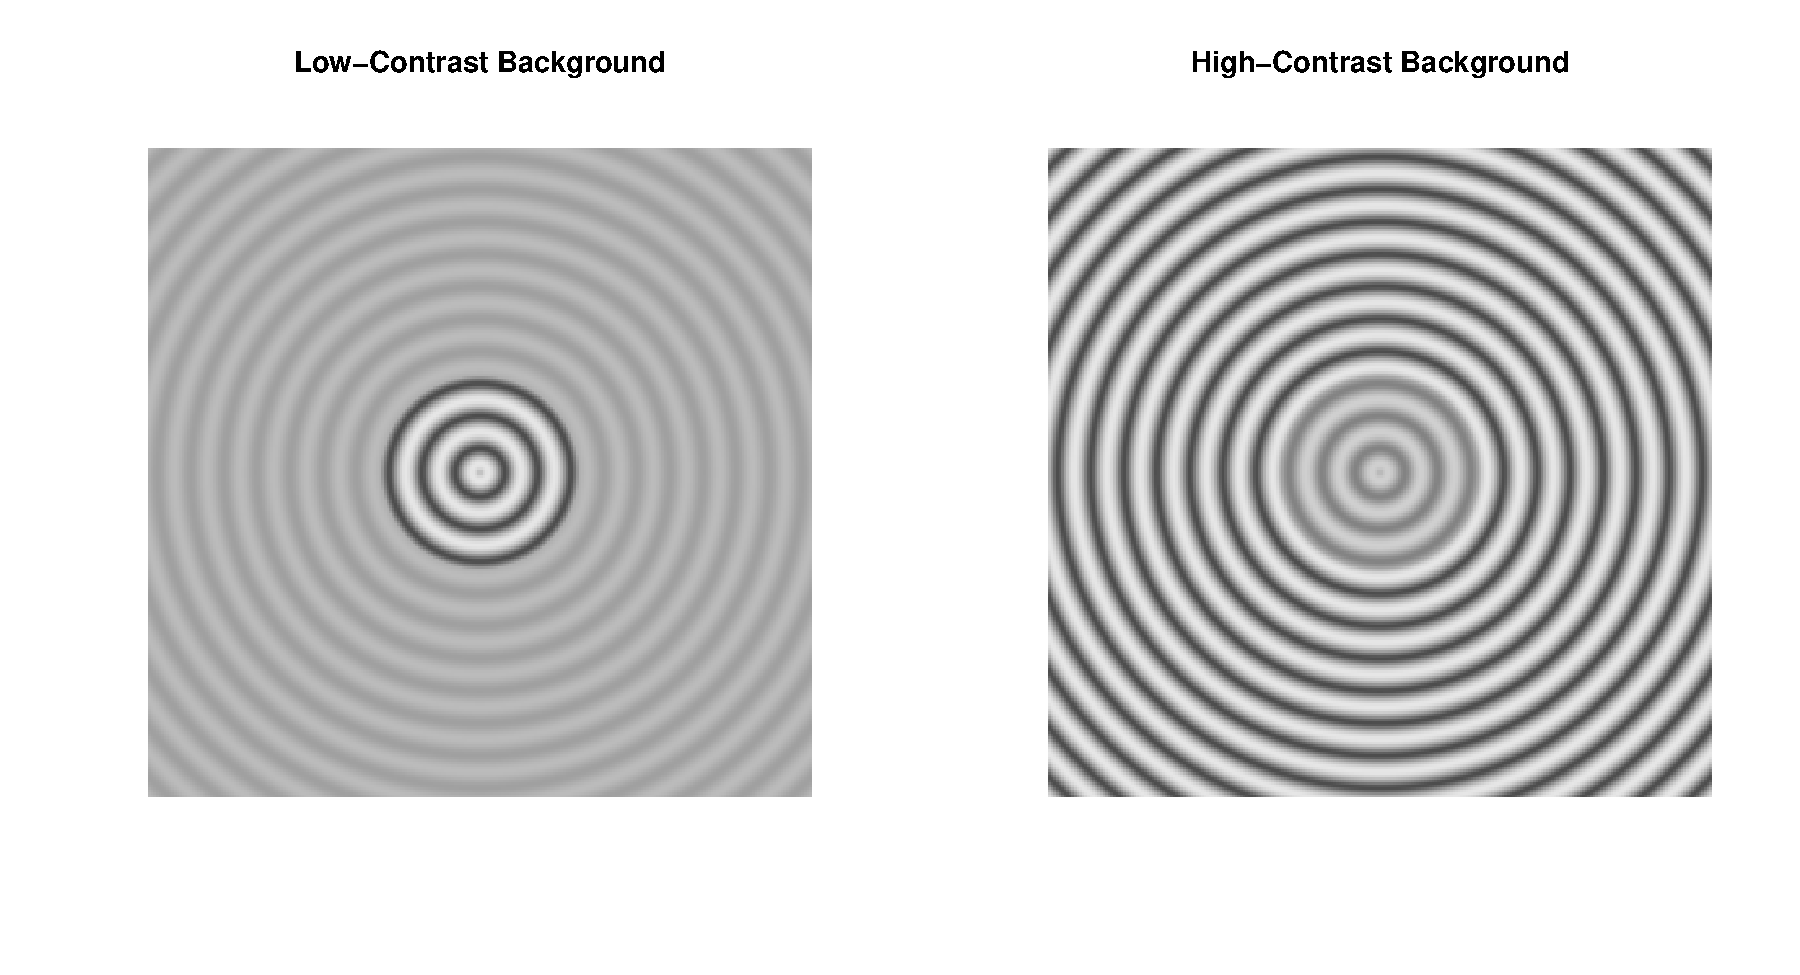
\includegraphics{Figures/centresurround.pdf}

}

\caption{\label{fig-centresurround}The perceived contrast of a stimulus
depends on its context. A high contrast surround reduces the apparent
contrast of the central `probe' region.}

\end{figure}%

A significant body of research into contrast processing is concerned
with how these normalization mechanisms depend on colour (Chen \emph{et
al.}, 2000), orientation (Foley, 1994), eye of origin (Legge, 1979;
Baker \emph{et al.}, 2007), spatial and temporal frequency (Meese \&
Baker, 2009), location (Polat \& Sagi, 1993; Tadin \emph{et al.}, 2003;
Petrov \emph{et al.}, 2005), age (Betts \emph{et al.}, 2005), and the
presence of neurological disorders (Porciatti \emph{et al.}, 2000; Tsai
\emph{et al.}, 2011). The SSVEP has proven to be invaluable in this
research because it provides an objective readout of contrast
representation at different stages of the visual system, and allows us
to `tag' the probe and background at separate frequencies.

Because it provides a direct read-out of neural population activity, the
SSVEP signal can reveal key features of neural signal transduction. For
example, by varying the peak stimulus contrast parametrically, a
`contrast vs response' function (CRF) can be measured - where the
`response' is typically defined as the amplitude of the SSVEP frequency
component at the stimulus frequency, or a low multiple thereof. This
corresponds closely to similar functions reported by studies measuring
single unit activity or local field potentials in the cortex (Shapley \&
Victor, 1980; Morrone \emph{et al.}, 1982). However the SSVEP has the
advantage that it is non-invasive, and so can be measured in awake,
behaving human participants.

To understand the utility of the contrast SSVEP, it is helpful to
identify the cascade of processing stages in the early visual system
that give rise to it. In the following section we illustrate how a
typical SSVEP signal measured over early visual cortex might contain
information about a large number of early visual computations.

\section{Contrast processing - linear and
nonlinear}\label{contrast-processing---linear-and-nonlinear}

Neurons have a limited dynamic range, yet they can transmit information
about visual stimuli that span many orders of magnitude. In the domain
of contrast, to some extent this is accomplished at a population level -
individual neurons typically implement a non-linear, sigmoidal CRF
transducer (Tolhurst \emph{et al.}, 1981; Albrecht \& Hamilton, 1982)
and different neurons exhibit peak sensitivity (defined as the maximum
slope of the function) at different contrast levels (Carandini \&
Heeger, 1994; Carandini \emph{et al.}, 1998; Busse \emph{et al.}, 2009).
A neuronal population will therefore span a sensitivity range greater
than any individual member.

Individual neurons at multiple stages of the visual hierarchy also
change their sensitivity depending on the average spatiotemporal
contrast energy of their environment. This ``normalisation'' process is
dynamic and nonlinear and is well-modeled by a hyperbolic ratio function
in which the response of each neuron is modulated by a local `gain pool'
composed of the summed responses of the local neuronal population
(Heeger, 1992; Busse \emph{et al.}, 2009; Carandini \& Heeger, 2011;
Baker \& Wade, 2017).

To understand these processes better, we will show how sinusoidal input
signals might be processed by the visual system to produce SSVEPs.
Figure~\ref{fig-linear} illustrates how sine waves of different
contrasts are processed in a linear system. The first panel shows the
input sine wave, which would be used to modulate stimulus amplitude over
time. Notice that there are five peaks in the waveform during the one
second sample, so the stimulation frequency is 5Hz (F1). The second
panel shows Fourier transform of the waveform, which contains a
substantial peak at this frequency. If we change the stimulus contrast
(i.e.~the amplitude of the waveform), the amplitude of the F1 component
increases linearly with contrast (right panel).

\begin{figure}

\centering{

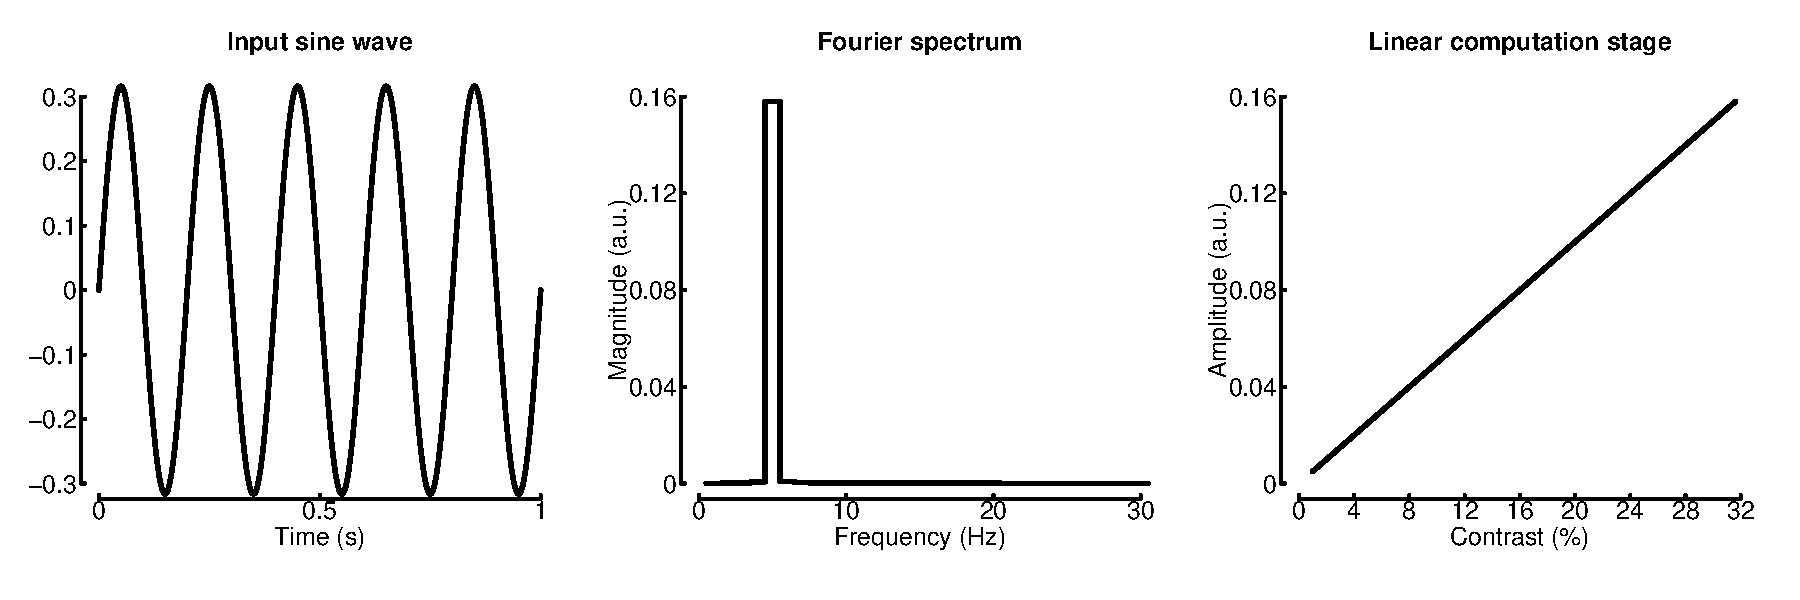
\includegraphics{Figures/linearsystem.pdf}

}

\caption{\label{fig-linear}Illustration of a sinusoidal input signal
(left), its Fourier spectrum (middle), and how the amplitude of the
first harmonic component increases with contrast (right). These
calculations assume an entirely linear system.}

\end{figure}%

Next we can consider the impact of a nonlinearity in processing on the
responses. One of the simplest nonlinearities is the function that
describes a cell's response to different levels of contrast. In
Figure~\ref{fig-transducer} this is modeled by a hyperbolic ratio
function resulting in a saturating non-linearity:

\begin{equation}\phantomsection\label{eq-nakarushton}{R_{\mathrm{max}} = \frac{C_{\mathrm{in}}^n}{C_{50}^n + C_{\mathrm{in}}^n},}\end{equation}

where \({R_{\mathrm{max}}}\) describes the maximum response level,
\(C_{\mathrm{in}}\) is the input contrast (or the time-varying
waveform), \(C_{50}\) is the `semi-saturation constant' (the point at
which the response is at half-maximum) and \emph{n} controls the
steepness of the curve (with a typical value around \(n=2\).

This nonlinearity has clear effects on signal transduction. The
sinusoidal waveform is distorted by the nonlinearity, and appears
frequency doubled (left panel of Figure~\ref{fig-transducer}; note that
other nonlinearities such as rectification and squaring can have similar
effects). The distortion is reflected in the Fourier spectrum (middle
panel of Figure~\ref{fig-transducer}), which now includes responses at
integer multiples (known as harmonics) of the stimulation frequency (10,
20 and 30Hz), but no response at the fundamental (5Hz). Finally, the
contrast response function is now nonlinear (right panel of
Figure~\ref{fig-transducer}). Although the hyperbolic ratio function
(Equation~\ref{eq-nakarushton}) is monotonic, the CRF resulting from
measuring the amplitude of the second harmonic (2F) component contains a
slight roll-off at high input contrasts. This results from the
distortion of the input sine waves at high contrast due to a combination
of the full-wave rectification and saturating non-linearity. Power at
other harmonics increases, and the total power generated by the input is
monotonic. This roll-off is often seen in experimental data and has been
referred to as `supersaturation' (Tyler \& Apkarian, 1985; Peirce,
2007).

\begin{figure}

\centering{

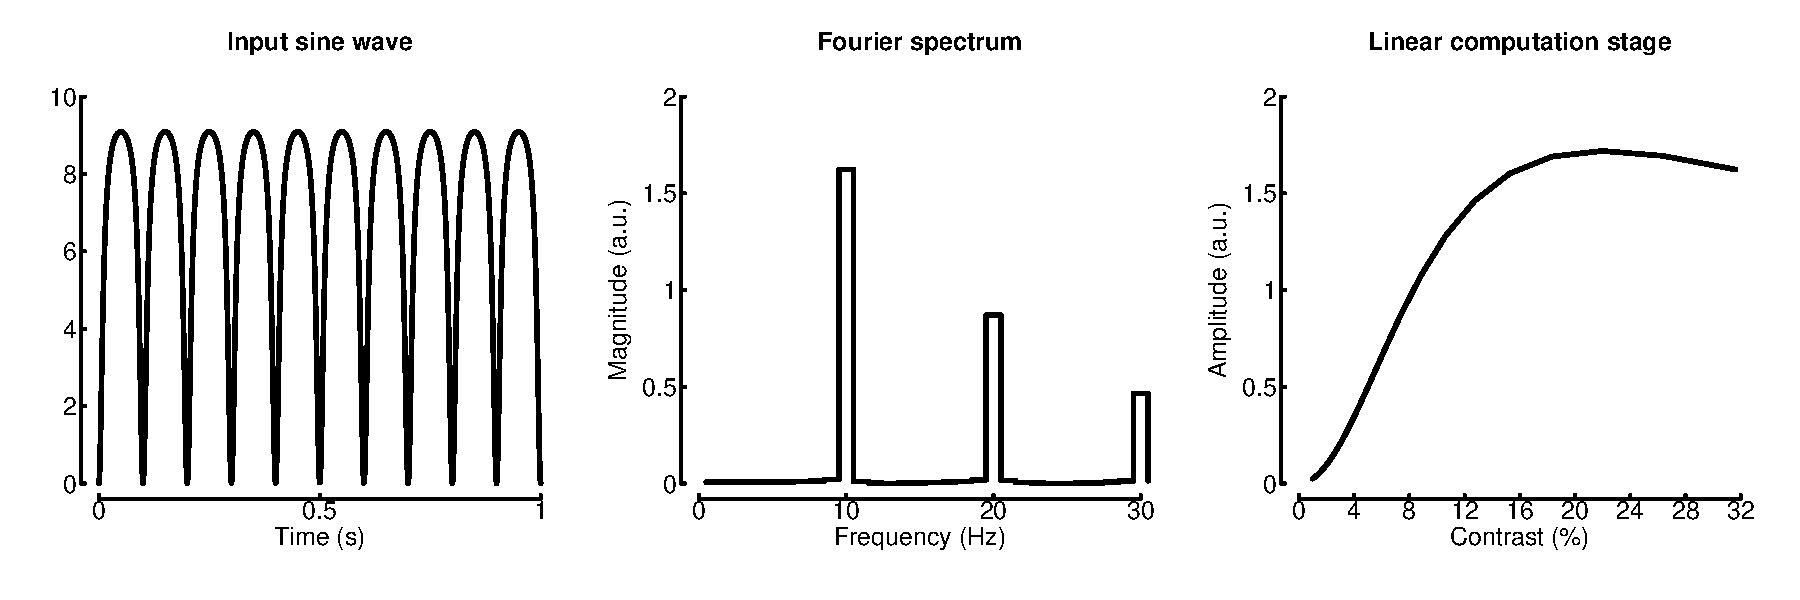
\includegraphics{Figures/transducer.pdf}

}

\caption{\label{fig-transducer}Illustration of how a sinusoidal input
signal is affected by a nonlinear transducer. The input wavefore (left
panel) is frequency doubled by the squaring operator, and now features
energy at the second harmonic (10Hz) and its multiple (middle panel).
The contrast response function at the second harmonic is now nonlinear,
and saturates at high contrasts (right panel).}

\end{figure}%

To illustrate the effect of contrast gain control (Heeger, 1992), we
next include a second component (a `mask') that contributes to the gain
pool of the first (the `target'). The mask stimulus will suppress the
response at the target frequency, reducing its amplitude. The
suppression is reciprocal - activity at the mask frequency is also
reduced by the presence of the target, in a contrast-dependent manner
(Busse \emph{et al.}, 2009). At a single pair of (matched) contrast
levels, we see a complex pattern of intermodulation terms in the
transduced waveforms (left panel of Figure~\ref{fig-twoinputs}) and in
the Fourier spectrum (middle panel of Figure~\ref{fig-twoinputs}). The
two components interact generating nonlinear intermodulation terms at
sums and differences of the input frequencies (F1, F2). The nature of
the interaction --- and therefore the pattern of intermodulation terms
--- is determined by the computations happening as the contrast signal
moves from retina to cortex (Regan \& Regan, 1988).

\begin{figure}

\centering{

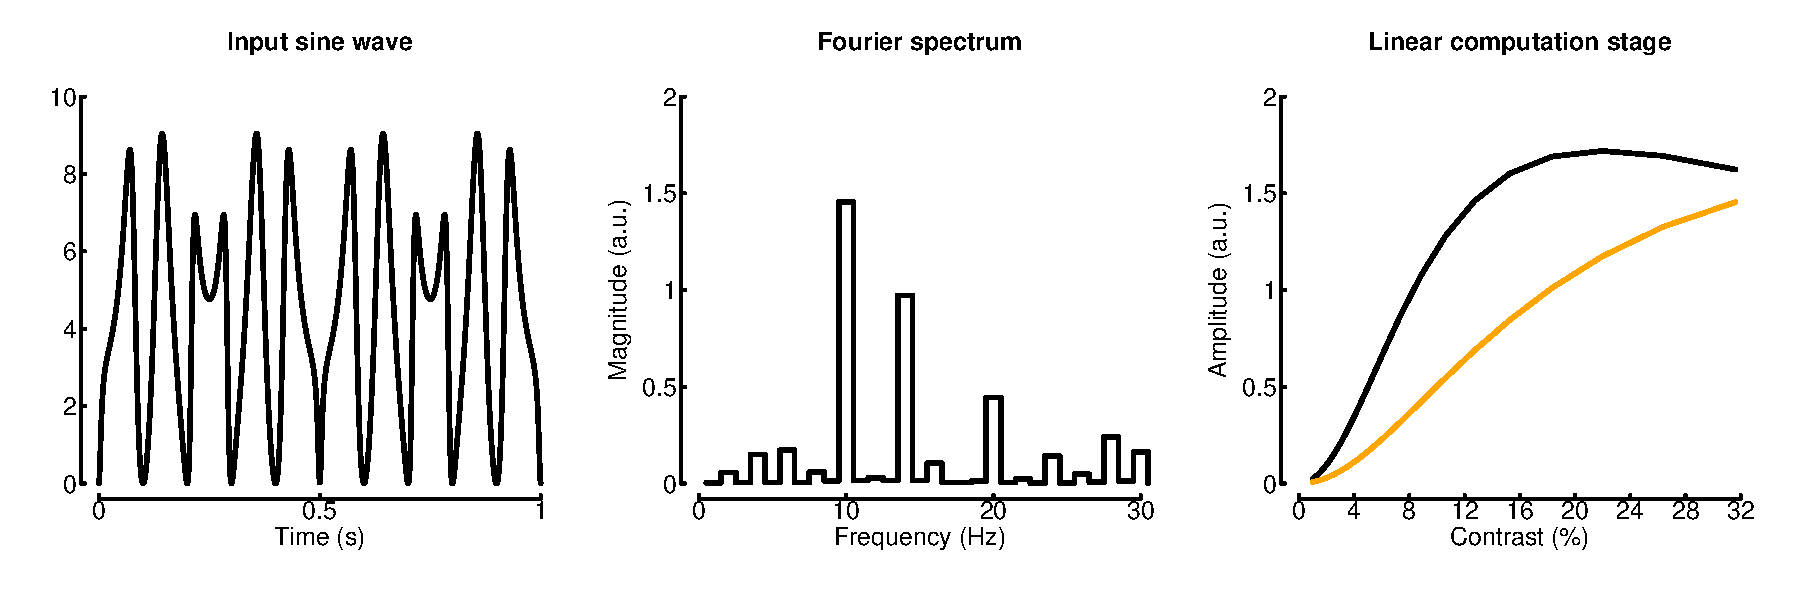
\includegraphics{Figures/twoinputs.pdf}

}

\caption{\label{fig-twoinputs}Demonstration of how two inputs of
different frequencies are processed by a nonlinear transducer.
Additional harmonics are apparent in the Fourier spectrum (middle
panel), and the contrast response function is suppressed (right panel).}

\end{figure}%

If the two inputs were simply added together, the representation of the
resulting signal in the Fourier domain would be the linear sum of the
two independent signals (i.e.~peaks at F1 and F2). However, it is
important to take physiology into account. Contrast gain control reduces
the amplitude of the responses via a suppressive process, which can be
incorporated into our transducer function via an additional denominator
term:

\begin{equation}\phantomsection\label{eq-gaincontrol}{R_{\mathrm{max}} = \frac{C_{\mathrm{in}}^n}{C_{50}^n + C_{\mathrm{in}}^n + C_{\mathrm{mask}}^n},}\end{equation}

where \(C_\mathrm{mask}\) reflects the contrast of the mask component at
a distinct frequency from that of the target. The effect of this extra
term is to reduce the target response (see right panel of
Figure~\ref{fig-twoinputs}). For a linear contrast axis, the contrast
response function becomes shallower, whereas on a logarithmic contrast
axis it maintains its steepness and shifts to the right. Suppressive
effects of this kind have been obtained using SSVEP with a variety of
different types of mask, including orthogonal overlaid masks, surround
masks, and dichoptic masks (Burr \& Morrone, 1987; Ross \& Speed, 1991;
Candy \emph{et al.}, 2001; Busse \emph{et al.}, 2009; Cunningham
\emph{et al.}, 2017; Salelkar \& Ray, 2020; for a meta-analysis see
Baker \emph{et al.}, 2021).

Even without considering a spatial component, the early visual system is
far more complex than the model here suggests. For example as well as
cells that code positive or negative contrast in a more or less
continuous manner, the retina also contains `transient' cells that code
temporal changes in contrast. These cells (Kuffler \emph{et al.}, 1957;
Alpern, 1971), and cells with similar properties in the LGN (Levitt
\emph{et al.}, 2001) and cortex (Hubel \& Wiesel, 1959; Movshon, 1975),
will introduce second harmonic components even when the stimulus itself
is modulated in an on-off fashion. Analogously, in the spatial domain,
so-called `simple cells' are sensitive to the polarity of a spatial
contrast modulation while `complex cells' respond to the presence of
patterned spatial contrast irrespective of its spatial position (Hubel
\& Wiesel, 1962). The SSVEP response to a contrast-reversing sine-wave
grating therefore contains information about nonlinear computations
performed across a range of retinal and cortical cell types.

The complexity of even a simple simulation of the frequency-domain
signal arising from non-linear interactions is intriguing. Presumably,
the signal measured from early visual cortex is the result of a cascade
of nonlinear retinal and cortical operations up to that point. It
therefore contains a `signature' or `fingerprint' of the computational
nature, order and parameters of those operations - including the shape
of the transducer functions and the computations involved in signal
combination. In principle, that information could be recovered from the
SSVEP signal - a possibility recognised in the early days of the
technique (Regan \& Regan, 1988). Although characterising the complete
set of computations along entire processing pathway is challenging,
careful parametric variation of the input stimuli does allow us to fit
models of early visual gain control using SSVEP data. For example, Tsai
\emph{et al.} (2012) demonstrated that a gain control model gave a good
account of the pattern of intermodulation responses produced by two
overlaid patterns flickering at different frequencies. This was achieved
by passing full stimulus waveforms through the transducer nonlinearity,
and calculating the Fourier spectrum of the model output. Our more
recent work on signal combination across eyes and space similarly
demonstrated close correspondence between the predictions of a
computational model and empirical data in humans (Baker \& Wade, 2017).
More detailed modelling of intracortical recordings (Groen \emph{et
al.}, 2022) has revealed details of the timecourse of gain control
effects, specifically that normalization is delayed slightly relative to
the initial visual response.

Similar changes to the contrast response function might also be obtained
using adaptation paradigms, in which the visual system is exposed to
high contrast stimuli for long durations. Psychophysically, adaptation
increases detection thresholds, but has little effect on contrast
discrimination performance (Ross \emph{et al.}, 1993), much like pattern
masks (Foley, 1994). Although SSVEP adaptation effects show strong
tuning for orientation (Campbell \& Maffei, 1970; Vergeer \emph{et al.},
2018) and spatial frequency (Mecacci \& Spinelli, 1976), there appear to
be no studies measuring the full SSVEP contrast response function before
and after an extended period of adaptation.

\section{Measuring the development of contrast
processing}\label{measuring-the-development-of-contrast-processing}

An early use of the SSVEP was to provide an objective estimate of
spatial contrast sensitivity in infants, without requiring behavioural
responses. In well-motivated adults, psychophysical measurements of
contrast sensitivity remain the gold standard. However, it is difficult
and time consuming to obtain reliable psychophysical data from infants.
In these cases, SSVEP measurements represent a fast and efficient method
for measuring low-level visual responses (Tyler \emph{et al.}, 1979;
Braddick \emph{et al.}, 1986; Norcia \emph{et al.}, 1990) and the high
SNR of SSVEP means that infants need only look at the screen for short
periods of time.

Because SSVEP responses at detection threshold are very small,
estimating a threshold is achieved by measuring the contrast response
function at relatively high levels, and extrapolating back along the
function (either contrast vs response measured at a constant spatial
frequency or spatial frequency vs response at a constant contrast level)
to estimate its intercept with the x-axis (see
Figure~\ref{fig-sweepvep}). This contrast level was shown to correspond
approximately with psychophysically measured detection thresholds
(Norcia \emph{et al.}, 1986).

\begin{figure}

\centering{

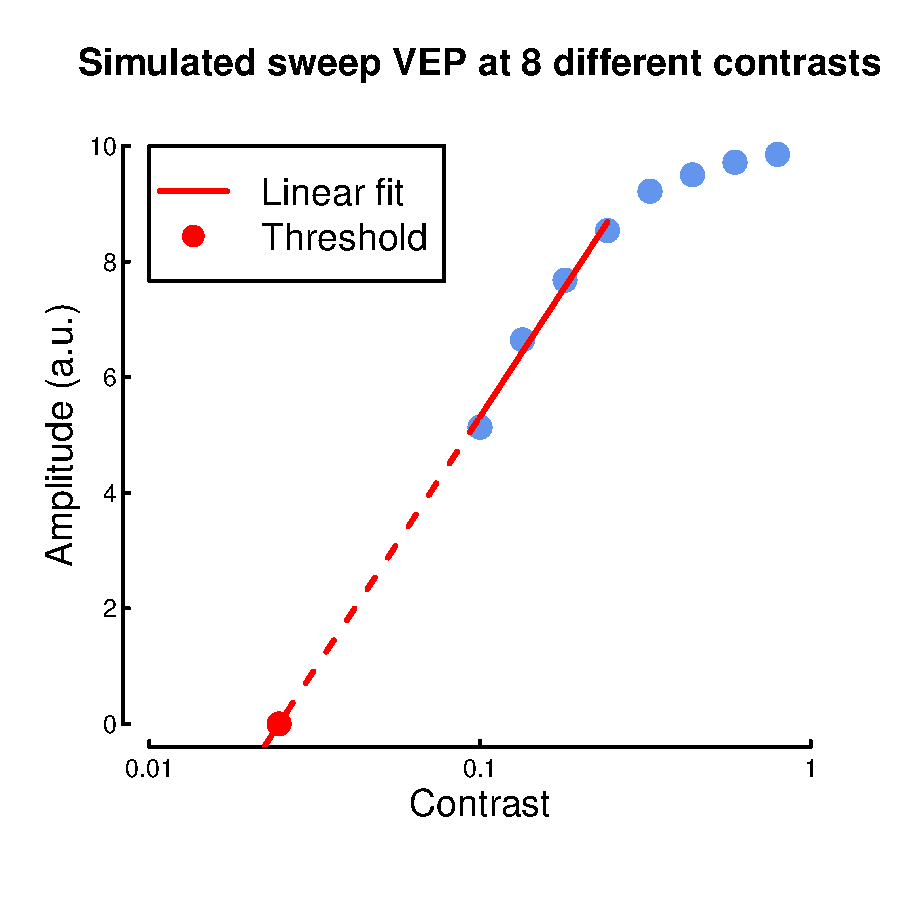
\includegraphics{Figures/sweepplot.pdf}

}

\caption{\label{fig-sweepvep}Sweep VEP simulation showing how a contrast
detection threshold can be estimated from sweep VEP data measured at
higher contrasts. The solid line is the regression fit to the lowest
four data points, and the dashed line extrapolates the fit back to
determine the contrast value when y=0, which gives a threshold estimate
(red point).}

\end{figure}%

A robust estimate of the threshold therefore requires the measurement of
the SSVEP amplitude at many different super-threshold contrast levels.
This was made faster by the development of the `sweep VEP' paradigm in
which the stimulus changed its contrast, spatial frequency or some other
property, throughout a trial (Tyler \emph{et al.}, 1979). To avoid
hysteresis effects, the sweep is sometimes conducted both up and down in
the same experiment (Tyler \emph{et al.}, 1979; Norcia \& Tyler,
1985\emph{a}; Norcia \emph{et al.}, 1990). The sweep VEP (really, a
sweep `SSVEP') technique is now commonly-used to obtain a rapid and
objective measurement of visual acuity. In particular, because of its
relative speed and simplicity, this technique has now become a standard
for conducting tests of visual acuity in very young subjects or where
behavioural tests are not appropriate (Ridder, 2004; Bach \emph{et al.},
2008; Hoffmann \emph{et al.}, 2017; Bach \& Farmer, 2020).

This approach has revealed much about the development of visual
abilities in infants (Harris \emph{et al.}, 1976; Atkinson \emph{et
al.}, 1979; Braddick \emph{et al.}, 1986). In general, SSVEP
measurements of infant vision have revealed that contrast sensitivity
for both achromatic and chromatic contrast as well as stereoscopic depth
perception develops earlier than had been supposed previously based on
behavioural readouts (Dobson \emph{et al.}, 1978; Norcia \& Tyler,
1985\emph{b}) with both chromatic and achromatic contrast detection
reaching near-adult levels by around six months. Spatial acuity as
measured by SSVEP reaches adult levels more slowly, but near-adult
levels are recorded around one year (Norcia \& Tyler, 1985\emph{b};
Hamer \emph{et al.}, 1989) compared to around six to seven years with
behavioural measures (Atkinson \& Braddick, 1983; Ellemberg \emph{et
al.}, 1999). At least some of this difference is likely due to the
relative objectivity and high SNR of the SSVEP technique compared to
other methods such as preferential looking, which require careful
measurement of the infant's gaze direction. However it should be noted
that other groups have reported electrophysiological correlates of
visual acuity that more closely match the behavioural measures (De
Vries-Khoe \& Spekreijse, 1982).

The SSVEP technique has also been used to study the development of the
contrast gain control mechanisms described in the previous section
(Candy \emph{et al.}, 2001; Pei \emph{et al.}, 2017). Although contrast
gain control is measurable in infants as young as six weeks old (Morrone
\& Burr, 1986; Skoczenski \& Norcia, 1998; Candy \emph{et al.}, 2001),
its development appears to be slower, with adult levels being reached at
approximately 11 years (Pei \emph{et al.}, 2017).

\section{Contrast processing in clinical
conditions}\label{contrast-processing-in-clinical-conditions}

The SSVEP technique has also been used to study clinical conditions,
such as diseases and developmental disorders. This can often be
informative regarding the underlying mechanism that characterises the
condition. Here we focus on four conditions, but there is potential to
apply the method more broadly: as a dignostic technique, to monitor
disease severity and progression, or to assess the efficacy of
treatments.

Epilepsy is a neurological condition in which patients experience
seizures - episodes of uncontrolled neural activity that can cause
unconsciousness, involuntary movements and convulsions, and atypical
sensory experiences. Porciatti \emph{et al.} (2000) showed that
individuals with photosensitive epilepsy generate larger steady-state
signals in response to flickering visual stimuli, and their contrast
response functions saturate less than those of healthy controls. This is
consistent with the idea that epilepsy involves a cortical
hyperexciteability that makes seizures more likely. It is also the case
for individuals with idiopathic generalised epilepsy (Tsai \emph{et
al.}, 2011), a subtype of epilepsy that has a less obvious link to
vision. The differences apply across the whole contrast-response
function, and so resemble a response gain effect (see
Figure~\ref{fig-plotclinical}a), which might be due to reduced
inhibition from neighbouring neurons. Differences in SSVEP amplitudes
have also been reported in individuals with migraine (Shibata \emph{et
al.}, 2008), a condition also associated with cortical
hyperexciteability.

Amblyopia is a disorder of binocular vision, characterised by one eye
contributing much less to perception than the other. This is often due
to strabismus (squint) or anisometropia (difference in optical
prescription between the eyes) during development. Contemporary accounts
suggest that the amblyopic eye is suppressed by signals from the fellow
eye. SSVEPs provide a convenient and objective method to characterise
the difference in neural response to signals in each eye, and typically
show reduced responses to stimuli in the amblyopic eye (see
Figure~\ref{fig-plotclinical}b) across the contrast range (Baker
\emph{et al.}, 2015; Lygo \emph{et al.}, 2021). There are currently many
novel binocular treatments for amblyopia under development, often
involving virtual reality or stereo display systems designed to
encourage the two eyes to work together. The steady-state approach may
be more sensitive and objective than typical acuity measurements, and
also has the potential to measure suppression between the eyes directly
(e.g. Zheng \emph{et al.}, 2019; Hu \emph{et al.}, 2023; Du \emph{et
al.}, 2023).

Autism is a condition often associated with differences in vision
(Simmons \emph{et al.}, 2009) and other senses (MacLennan \emph{et al.},
2022). Pei \emph{et al.} (2014) used a sweep-VEP method with
counterphase flickering stimuli, and found weaker responses in autistic
children at spatial frequencies around 8c/deg, compared with age-matched
controls. This was subsequently replicated in a further pediatric sample
by Vilidaite \emph{et al.} (2018) (see Figure~\ref{fig-plotclinical}c),
who additionally found weaker responses in autistic adults at the second
harmonic (using on/off flicker). Interestingly this study replicated its
key findings in a \emph{Drosophila} genetic model of autism (\emph{Nhe3}
mutations), illustrating the translational potential of the steady-state
approach, as well as identifying a possible biomarker for autism.

Recent work on understanding Parkinson's disease has also used
\emph{Drosophila} genetic models. Afsari \emph{et al.} (2014) found that
mutant flies produced stronger SSVEP responses to flickering lights than
control flies (see Figure~\ref{fig-plotclinical}d). The authors
theorised that differences in early gain control during development
might lead to visual deficits later in life. Although visual responses
are a convenient assay of neural function, it is likely that the same
general process applies throughout the whole brain, including in the
motor system where the core Parkinson's symptoms (tremor, rigidity, slow
movement) manifest. The SSVEP differences were reduced by a kinase
inhibitor that targets the dopamine system, demonstrating how model
organisms can be used to test new pharmacological treatments. SSVEP
responses also provide a potential method to diagnose Parkinson's before
any symptoms manifest, and to monitor the effect of treatments.

\begin{figure}

\centering{

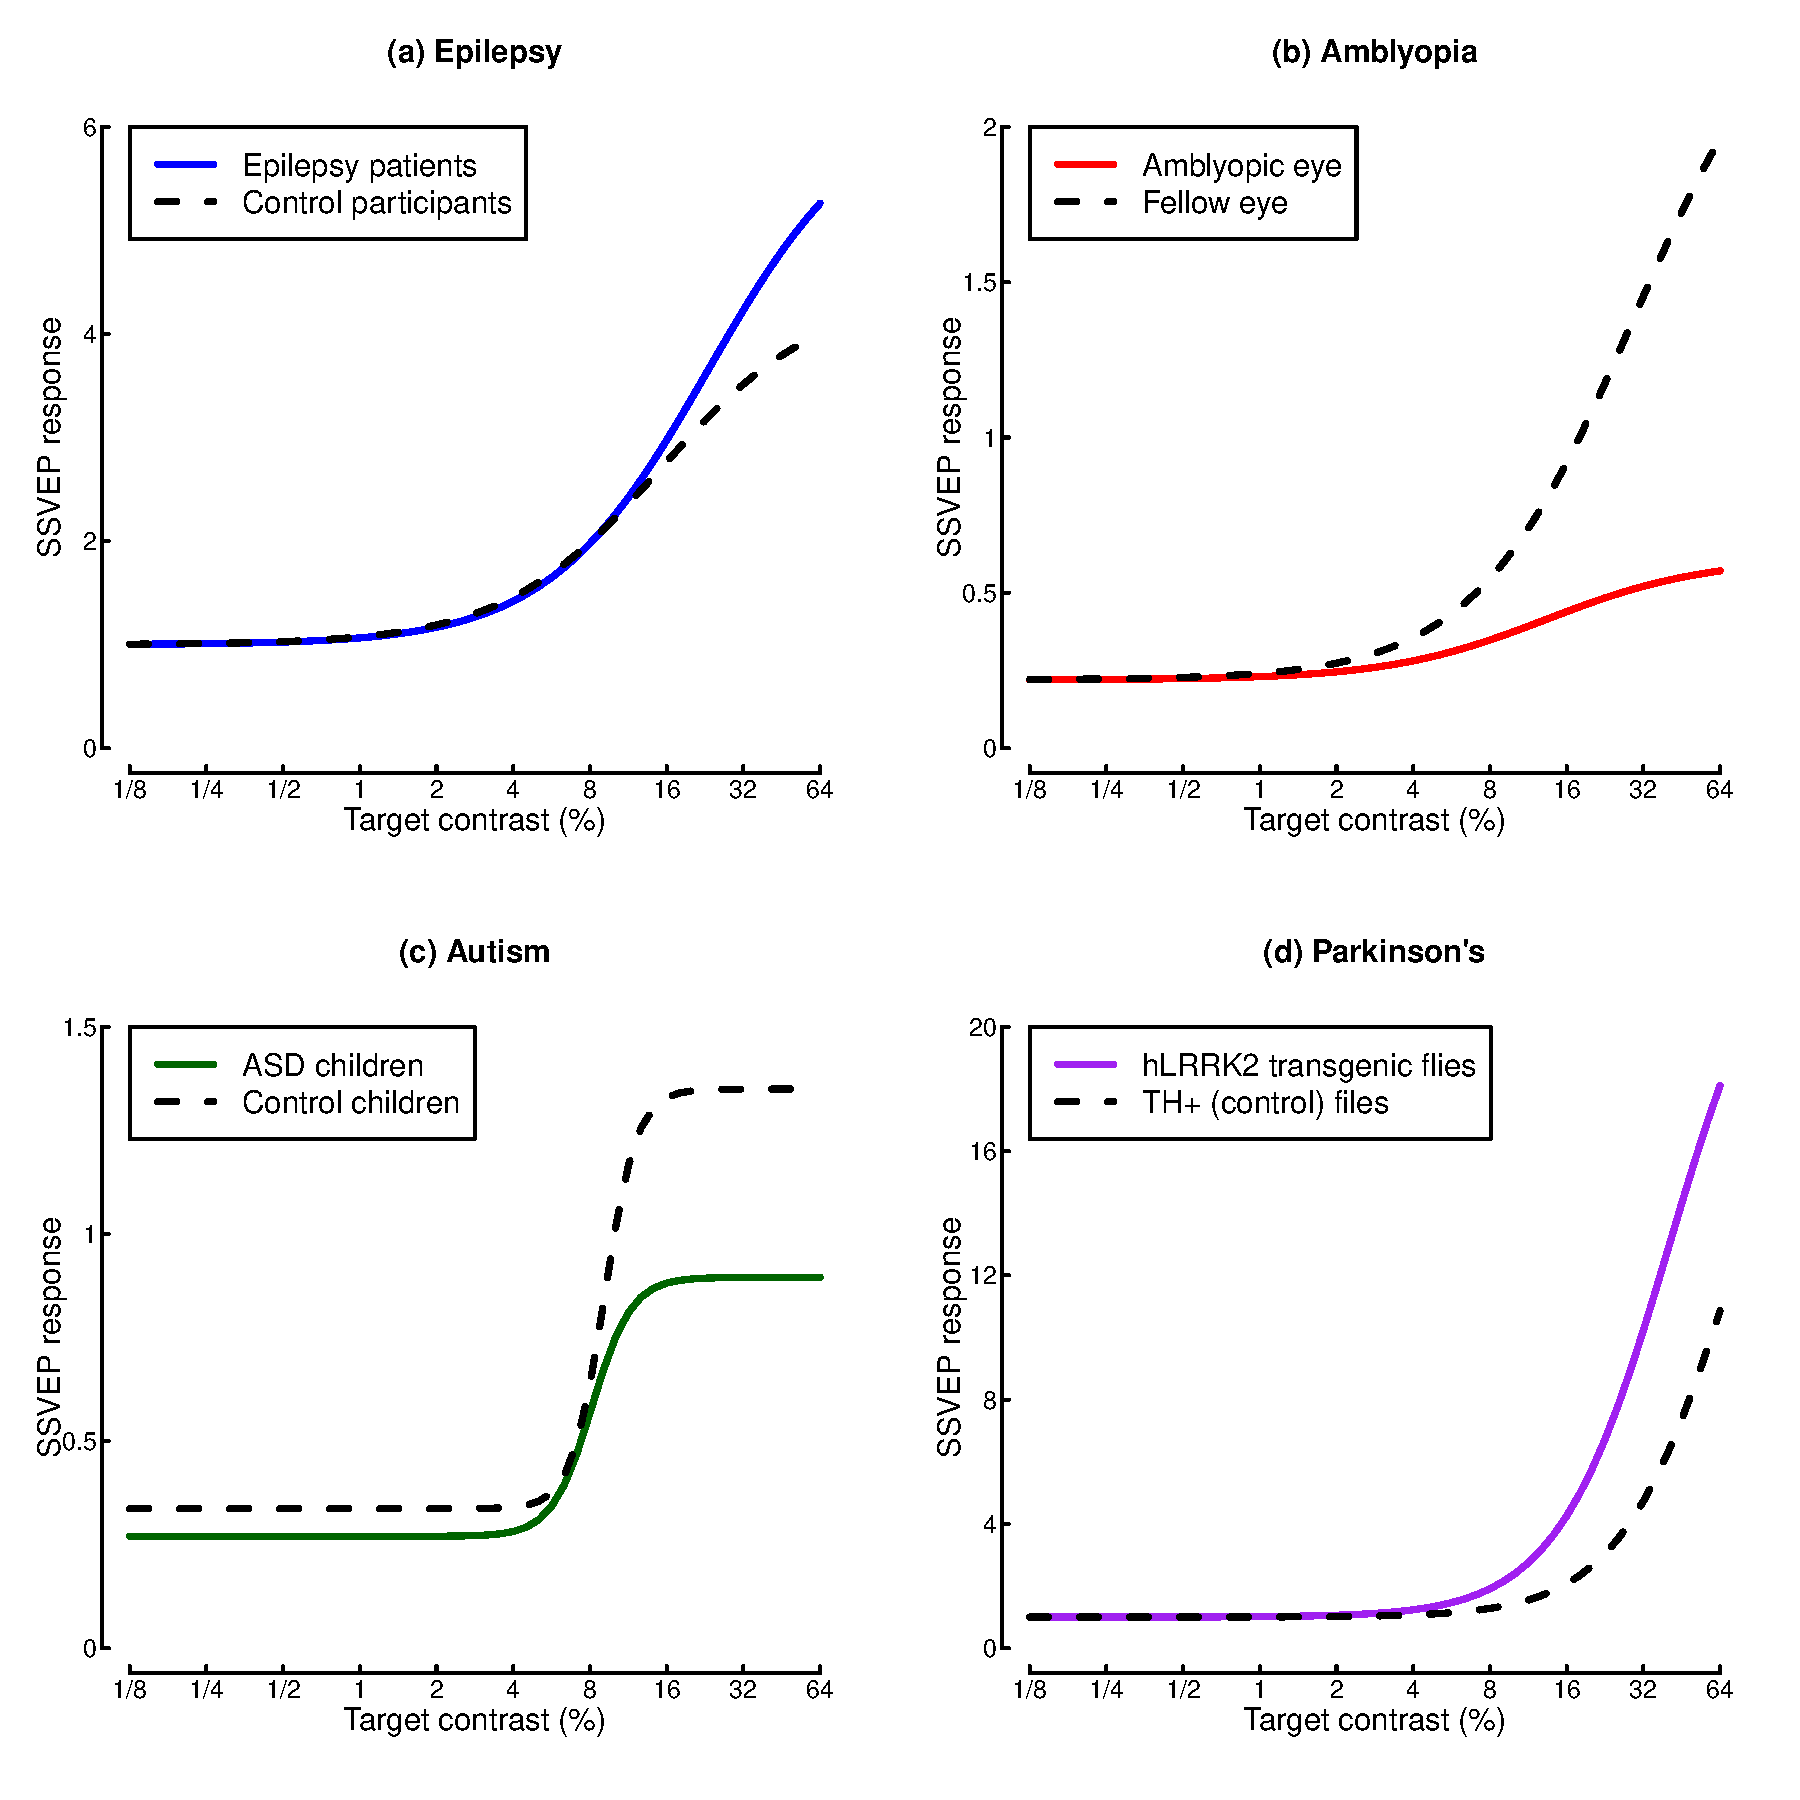
\includegraphics{Figures/clinicalplot.pdf}

}

\caption{\label{fig-plotclinical}Example contrast response functions for
different clinical conditions. Panel (a) shows modelled contrast
response functions for epilepsy patients (blue) and control participants
(black), based on the data of Tsai et al.~(2011). Panel (b) shows
functions for the amblyopic (red) and fellow (black) eyes of adults with
amblyopia, based on the data of Baker et al.~(2015). Panel (c) shows
functions for children with (green) and without (black) a diagnosis of
autism, based on the data of Vilidaite et al.~(2018). Panel (d) shows
data from \emph{Drosophila melanogaster} (fruit flies) from Afsari et
al.~(2014). One day-old flies expressing a human gene linked to
Parkinson's (hLRRK-G2019S) show increased SSVEP response amplitude and
sensitivity (red) compared to control animals (black).}

\end{figure}%

\section{Attention and arousal}\label{attention-and-arousal}

Attention exerts a profound influence on visual performance: for
example, instructing people to attend covertly to a spatial location
improves their performance on a target detection task significantly
(Bashinski \& Bacharach, 1980; Posner, 1980; Carrasco \emph{et al.},
2000; Cameron \emph{et al.}, 2002; Morrone \emph{et al.}, 2004; Pestilli
\emph{et al.}, 2009). In principle, this enhancement may be driven both
by modulation of the underlying signal or noise characteristics, or by
additional decision-theoretic factors such as reduction in spatial
uncertainty (Petrov \emph{et al.}, 2006; Gould \emph{et al.}, 2007).
Early experiments with non-human primates showed little evidence for
attentionally-driven changes in neuronal spike rates (Luck \emph{et
al.}, 1997; McAdams \& Maunsell, 1999; Mehta \emph{et al.},
2000\emph{a}, 2000\emph{b}; Marcus \& Van Essen, 2002), but with the
advent of spatially-resolved human brain imaging methods in the late
1990s it became apparent that spatial attention was linked to frank
changes in both fMRI BOLD responses (Tootell \emph{et al.}, 1998; Somers
\emph{et al.}, 1999; Gandhi \emph{et al.}, 1999; Brefczynski \& DeYoe,
1999; Kastner \emph{et al.}, 1999; Buracas \& Boynton, 2007; Silver
\emph{et al.}, 2007; Li \emph{et al.}, 2008; Murray, 2008) and EEG
signals (Morgan \emph{et al.}, 1996; Müller \emph{et al.}, 1998; Müller
\& Hillyard, 2000; Ding \emph{et al.}, 2006).

Electrophysiological and psychophysical measurements of the effect of
attention on both luminance and chromatic contrast have strongly
implicated gain control as an underlying mechanism (Lu \& Dosher, 1998;
Di Russo \& Spinelli, 1999\emph{a}; Di Russo \emph{et al.},
2001\emph{b}). These effects also appear to differ between chromatic and
achromatic pathways (Di Russo \& Spinelli, 1999\emph{b}) - perhaps as a
result of the different levels of nonlinear gain control in the early
pre-cortical magno-, parvo- and konio-cellular pathways (Derrington \&
Lennie, 1984; Kaplan \& Shapley, 1986; Lee \emph{et al.}, 1990; Solomon
\& Lennie, 2005). In the late 2000s a comprehensive theoretical model
for attentional modulation was developed that framed it as a gain
control computation (Reynolds \& Heeger, 2009; Boynton, 2009). This
framework has proven to be influential - explaining a wide range of
phenomena from the earlier literature and demonstrating subtle
interactions between the size of the attentional `spotlight' and the
stimulus configuration which rationalise many apparent contradictions in
the literature. Direct measurements of attentional modulation of
achromatic SSVEP signals are broadly consistent with this model
(Lauritzen \emph{et al.}, 2010; Hou \emph{et al.}, 2016; Martinovic \&
Andersen, 2018) and confirm the relatively weaker role of spatial
attention on responses driven by chromatic stimuli - particularly those
that isolate the opponent S-(L+M) cone pathway (Highsmith \& Crognale,
2010; Wang \& Wade, 2011). The gain control model of attention can also
be extended to SSVEP studies of feature-based attention which show that
the modulatory effects can be targeted to the most informative neuronal
populations (Verghese \emph{et al.}, 2012).

The SSVEP can also be used to study changes in visual processing
\textit{driven} by different behavioural states or overall arousal. For
example, locomotion has been shown to alter neuronal excitability and
spatial normalization in mice (Niell \& Stryker, 2010; Ayaz \emph{et
al.}, 2013) - running mice have higher visual sensitivity and lower
surround suppression compared to stationary mice. Although measuring EEG
responses from locomoting humans is technically challenging, SSVEP
studies (which are able to distinguish broadband noise from input signal
effectively) have shown that walking also alters early visual
processing, although in a manner different to that observed in mice
(Benjamin \emph{et al.}, 2018; Cao \& Händel, 2019).

SSVEP measurements are typically used to measure time-invariant
responses due to sustained attention. However, recent work has shown
that moderately high modulation frequencies (ca 10Hz) and short analysis
windows (1.5s) can also be used to track the dynamic allocation of
attention across a task (Chota \emph{et al.}, 2024) or attention to
moving targets (Lissa \emph{et al.}, 2020). The ability to track changes
in attention over short time periods is also important if SSVEP is to be
used for dynamic readouts - for example in a Brain Computer Interface.

\section{Brain-computer interfaces}\label{brain-computer-interfaces}

One widespread recent application of the SSVEP technique is in the
design of brain-computer interfaces, which seek to control some aspect
of a computer using neural signals. The high SNR and precise frequency
resolution of SSVEPs are advantages for this approach. Typical studies
may involve presenting an array of stimuli at different flicker
frequencies, and having the participant select one either by overt
attention (i.e.~shifting fixation to foveate the selected stimulus) or
covert attention (i.e.~deploying attention to one stimulus whilst
keeping fixated) (Middendorf \emph{et al.}, 2000). Because SSVEP signals
are highly sensitive to both visual field position (Di Russo \emph{et
al.}, 2007; Ales \emph{et al.}, 2010) and attentional state (Morgan
\emph{et al.}, 1996; Müller \emph{et al.}, 1998; Lauritzen \emph{et
al.}, 2010; Verghese \emph{et al.}, 2012), the response to the selected
stimulus will typically increase relative to the others, allowing it to
be identified by an on-line algorithm. Because more than one stimulus
frequency is generally present, this modulation and the associated
changes in gain control will affect the entire pattern of self- and
intermodulation terms, allowing the choice to be decoded by a
multivariate pattern classifier.

This approach is primarily useful in situations that require the BCI to
distinguish from among a small set of possibilties: for example, in
early work, visual stimuli representing `Left' and `Right' commands in a
flight simulator were distinguished robustly (Middendorf \emph{et al.},
2000). Although SSVEP-based BCI interfaces typically do use contrast
flicker, work in this field has largely focused on optimising the
stimuli or decoders to increase decoding performance and reducing visual
fatigue associated with the long-term presentation of arrays of
high-contrast flicker (Diez \emph{et al.}, 2024), rather than studying
visual contrast processing \textit{per se}. We therefore note in passing
that using SSVEPs to improve our understanding of early contrast
processing may yield benefits to this related field.

\section{Future directions}\label{future-directions}

The SSVEP is a powerful tool for studying contrast processing. It
provides a high SNR readout of neuronal activity that is unambigously
linked to the input. It is sensitive to both the amplitude and phase of
the input and when combined with source imaging, it can be extracted
from different cortical regions allowing researchers to track contrast
processing computations across the visual pathway. Because of the high
SNR, it can be measured in subjects where long recording durations are
impractical (for example, infants or patients with neurological
disorders) and at frequencies high enough to be effectively invisible
(Herrmann, 2001; Seijdel \emph{et al.}, 2023; Minarik \emph{et al.},
2023). The SSVEP is also able to `fingerprint' modulators of the inputs
through the harmonic and intermodulation terms they generate in the
output. In principle, each nonlinearity in the visual pathway can be
identified by its contribution to the frequency spectrum at different
recording locations (Regan \& Regan, 1988). This, it turn, allows
researchers to study how contrast processing depends on spatial and
temporal context, as well as changes in task, cognitive and behavioural
state, and arousal.

Although visual neuroscience is a relatively old subfield, there are
still outstanding questions relating to contrast processing that could
be addressed by SSVEP methods. First, it is still not completely clear
how contrast signals are computed in the human retina. Although we have
more than a century of electrophysiological data from animals, and the
broad structure of cone inputs to retinal ganglion cells is understood
(Li \emph{et al.}, 2014), we are still discovering new aspects of
retinal processing that could influence the `coining' of the visual
system's currency (Gollisch \& Meister, 2010; Uprety \emph{et al.},
2022; Wang \emph{et al.}, 2023). The ability to frequency tag both
inputs (for example, cone-directed luminance contrast) and modulators
(for example, stimuli that selectively drive the
intrinsically-photosensitive retinal ganglion cells) is a powerful tool
to explore this first stage of image generation.

Later in the visual pathway, we would like to know more about the role
of corticothalamic feedback in the LGN. Although it is commonly thought
of as a simple relay between the eye and the cortex, the majority of
inputs to the LGN come from cortex not the eye, and there is good
evidence that contrast processing in the LGN can be altered by top-down
signals including attention (Sherman \& Guillery, 1996; O'Connor
\emph{et al.}, 2002; Briggs \& Usrey, 2007; Gouws \emph{et al.}, 2014).
Bottom-up inputs to the LGN are segregated by eye and so responses there
are often considered to be purely monocular, but it is possible that
feedback signals allow some binocular computations such as interocular
normalisation (Baker \emph{et al.}, 2007; Dougherty \emph{et al.}, 2019)
to begin even at this relatively early stage. Frequency tagging inputs
to different eyes or in different precortical pathways allows us to
address neurons in different parts of the LGN. These techniques combined
with advances in recording technology (for example, sensitive
source-imaged EEG and MEG recordings that can resolve subcortical
structures (Tesche, 1996; Attal \emph{et al.}, 2012; Attal \& Schwartz,
2013), noninvasive deep-brain stimulation techniques (Mohammadjavadi
\emph{et al.}, 2022) or implanted electrode arrays (Krolak-Salmon
\emph{et al.}, 2003)) may allow us to study these computations in more
detail.

Finally, SSVEPs continue to provide a way of studying contrast in the
cortex. Here, we are often interested in how different visual parameters
interact. For example, how are signals from different eyes combined to
generate both scalar contrast values and also binocular depth cues? How
does contrast combination depend on the low level properties of the
individual inputs such as their retinotopic location, cone contrast,
spatiotemporal frequency, eye of origin and orientation? Colour vision
scientists are particularly interested in how chromatic signals
originating in a small number of cone-opponent retinal pathways are
transformed into a perceptual colour space where the `unique hues'
appear to be only weakly-related to the early retinal outputs and how
these computations are conditioned by the spatial and temporal
properties of the scene (Wandell, 1993; Gegenfurtner, 2003; Solomon \&
Lennie, 2007; Stoughton \& Conway, 2008; Kaneko \emph{et al.}, 2020; Li
\emph{et al.}, 2022). All of these questions can be addressed by using
SSVEP and frequency tagging to examine the computations that combine and
transform the inputs at different cortical stages (Busse \emph{et al.},
2009; Baker \& Wade, 2017; Katyal \emph{et al.}, 2018; Chen \&
Gegenfurtner, 2021; Watts \emph{et al.}, 2024). The original promise of
the SSVEP approach was that the entire complex-valued frequency spectrum
recorded at each location provided detailed information about the
processing nonlinearities up to and including that point. In principle,
this would allow researchers to uniquely fit the parameters of their
computational models of visual processing (Regan \& Regan, 1988). To
date, the complexity of the neuronal computations at even the earliest
stage of visual processing have hampered this effort - researchers
typically restrict their analyses to the amplitudes of single, low-order
frequency components (for example, the input frequencies or simple sums
and differences of those frequencies). As our understanding of the early
visual system improves, it is becoming possible to generate more
realistic parameterised forward models of signal generation (Tsai
\emph{et al.}, 2012; Baker \& Wade, 2017; Chariker \emph{et al.}, 2020;
Schrimpf \emph{et al.}, 2020; Groen \emph{et al.}, 2022). Feeding
frequency-tagged inputs into these types of model allows us to generate
synthetic SSVEP responses that can be compared with those measured in
human subjects. In principle, we are therefore able to use the SSVEP to
fit the parameters of early visual processing. This approach may also
allow us to develop more sensitive tests for the changes in early visual
processing that accompany a wide range of neurological diseases and
disorders.

\section*{References}\label{references}
\addcontentsline{toc}{section}{References}

\phantomsection\label{refs}
\begin{CSLReferences}{1}{1}
\bibitem[\citeproctext]{ref-Afsari2014}
Afsari F, Christensen KV, Smith GP, Hentzer M, Nippe OM, Elliott CJH \&
Wade AR (2014). \href{https://doi.org/10.1093/hmg/ddu159}{Abnormal
visual gain control in a {Parkinson}'s disease model}. \emph{Human
Molecular Genetics} \textbf{23,} 4465--4478.

\bibitem[\citeproctext]{ref-Albrecht1982}
Albrecht DG \& Hamilton DB (1982).
\href{https://doi.org/10.1152/jn.1982.48.1.217}{Striate cortex of monkey
and cat: Contrast response function}. \emph{J Neurophysiol} \textbf{48,}
217--237.

\bibitem[\citeproctext]{ref-Ales2010}
Ales JM, Yates JL \& Norcia AM (2010).
\href{https://doi.org/10.1016/j.neuroimage.2010.05.016}{V1 is not
uniquely identified by polarity reversals of responses to upper and
lower visual field stimuli}. \emph{Neuroimage} \textbf{52,} 1401--1409.

\bibitem[\citeproctext]{ref-Alpern1971}
Alpern M (1971).
\href{https://doi.org/10.1113/jphysiol.1971.sp009580}{Rhodopsin kinetics
in the human eye}. \emph{J Physiol} \textbf{217,} 447--471.

\bibitem[\citeproctext]{ref-Atkinson1983}
Atkinson J \& Braddick O (1983).
\href{https://doi.org/10.1111/j.1755-3768.1983.tb03927.x}{Assessment of
visual acuity in infancy and early childhood}. \emph{Acta Ophthalmol
Suppl} \textbf{157,} 18--26.

\bibitem[\citeproctext]{ref-Atkinson1979}
Atkinson J, Braddick O \& French J (1979).
\href{https://www.ncbi.nlm.nih.gov/pubmed/761974}{Contrast sensitivity
of the human neonate measured by the visual evoked potential}.
\emph{Invest Ophthalmol Vis Sci} \textbf{18,} 210--213.

\bibitem[\citeproctext]{ref-Attal2012}
Attal Y, Maess B, Friederici A \& David O (2012).
\href{https://doi.org/10.1515/rns.2011.056}{Head models and dynamic
causal modeling of subcortical activity using
magnetoencephalographic/electroencephalographic data}. \emph{Rev
Neurosci} \textbf{23,} 85--95.

\bibitem[\citeproctext]{ref-Attal2013}
Attal Y \& Schwartz D (2013).
\href{https://doi.org/10.1371/journal.pone.0059856}{Assessment of
subcortical source localization using deep brain activity imaging model
with minimum norm operators: A MEG study}. \emph{PLoS One} \textbf{8,}
e59856.

\bibitem[\citeproctext]{ref-Ayaz2013}
Ayaz A, Saleem AB, Schölvinck ML \& Carandini M (2013).
\href{https://doi.org/10.1016/j.cub.2013.04.012}{Locomotion controls
spatial integration in mouse visual cortex}. \emph{Curr Biol}
\textbf{23,} 890--894.

\bibitem[\citeproctext]{ref-Bach2020}
Bach M \& Farmer JD (2020).
\href{https://doi.org/10.1007/s10633-019-09726-2}{Evaluation of the
"freiburg acuity VEP" on commercial equipment}. \emph{Doc Ophthalmol}
\textbf{140,} 139--145.

\bibitem[\citeproctext]{ref-Bach2008}
Bach M, Maurer JP \& Wolf ME (2008).
\href{https://doi.org/10.1136/bjo.2007.130245}{Visual evoked
potential-based acuity assessment in normal vision, artificially
degraded vision, and in patients}. \emph{Br J Ophthalmol} \textbf{92,}
396--403.

\bibitem[\citeproctext]{ref-Baker2007}
Baker DH, Meese TS \& Summers RJ (2007).
\href{https://doi.org/10.1016/j.neuroscience.2007.01.030}{Psychophysical
evidence for two routes to suppression before binocular summation of
signals in human vision}. \emph{Neuroscience} \textbf{146,} 435--448.

\bibitem[\citeproctext]{ref-Baker2015}
Baker DH, Simard M, Saint-Amour D \& Hess RF (2015).
\href{https://doi.org/10.1167/iovs.14-15611}{Steady-state contrast
response functions provide a sensitive and objective index of amblyopic
deficits}. \emph{Invest Ophthalmol Vis Sci} \textbf{56,} 1208--1216.

\bibitem[\citeproctext]{ref-Baker2021}
Baker DH, Vilidaite G \& Wade AR (2021).
\href{https://doi.org/10.1371/journal.pcbi.1009507}{Steady-state
measures of visual suppression}. \emph{PLoS computational biology}
\textbf{17,} e1009507.

\bibitem[\citeproctext]{ref-Baker2017}
Baker DH \& Wade AR (2017).
\href{https://doi.org/10.1093/cercor/bhw395}{Evidence for an {Optimal}
{Algorithm} {Underlying} {Signal} {Combination} in {Human} {Visual}
{Cortex}}. \emph{Cerebral Cortex (New York, NY: 1991)} \textbf{27,}
254--264.

\bibitem[\citeproctext]{ref-Baseler1997}
Baseler HA \& Sutter EE (1997).
\href{https://doi.org/10.1016/s0042-6989(96)00209-x}{M and p components
of the VEP and their visual field distribution}. \emph{Vision Res}
\textbf{37,} 675--690.

\bibitem[\citeproctext]{ref-Bashinski1980}
Bashinski HS \& Bacharach VR (1980). Enhancement of perceptual
sensitivity as the result of selectively attending to spatial locations.
\emph{Perception \& psychophysics} \textbf{28,} 241--248.

\bibitem[\citeproctext]{ref-Benjamin2018}
Benjamin AV, Wailes-Newson K, Ma-Wyatt A, Baker DH \& Wade AR (2018).
\href{https://doi.org/10.1523/JNEUROSCI.1428-17.2017}{The {Effect} of
{Locomotion} on {Early} {Visual} {Contrast} {Processing} in {Humans}}.
\emph{Journal of Neuroscience} \textbf{38,} 3050--3059.

\bibitem[\citeproctext]{ref-Betts2005}
Betts LR, Taylor CP, Sekuler AB \& Bennett PJ (2005).
\href{https://doi.org/10.1016/j.neuron.2004.12.041}{Aging reduces
center-surround antagonism in visual motion processing}. \emph{Neuron}
\textbf{45,} 361--366.

\bibitem[\citeproctext]{ref-Boynton2009}
Boynton GM (2009). \href{https://doi.org/10.1016/j.visres.2008.11.001}{A
framework for describing the effects of attention on visual responses}.
\emph{Vision Res} \textbf{49,} 1129--1143.

\bibitem[\citeproctext]{ref-Braddick1986}
Braddick OJ, Wattam-Bell J \& Atkinson J (1986).
\href{https://doi.org/10.1038/320617a0}{Orientation-specific cortical
responses develop in early infancy}. \emph{Nature} \textbf{320,}
617--619.

\bibitem[\citeproctext]{ref-Brefczynski1999}
Brefczynski JA \& DeYoe EA (1999). \href{https://doi.org/10.1038/7280}{A
physiological correlate of the 'spotlight' of visual attention}.
\emph{Nat Neurosci} \textbf{2,} 370--374.

\bibitem[\citeproctext]{ref-Briggs2007}
Briggs F \& Usrey WM (2007).
\href{https://doi.org/10.1523/JNEUROSCI.1035-07.2007}{A fast, reciprocal
pathway between the lateral geniculate nucleus and visual cortex in the
macaque monkey}. \emph{J Neurosci} \textbf{27,} 5431--5436.

\bibitem[\citeproctext]{ref-Buracas2007}
Buracas GT \& Boynton GM (2007).
\href{https://doi.org/10.1523/JNEUROSCI.3162-06.2007}{The effect of
spatial attention on contrast response functions in human visual
cortex}. \emph{J Neurosci} \textbf{27,} 93--97.

\bibitem[\citeproctext]{ref-Burr1987}
Burr DC \& Morrone MC (1987).
\href{https://doi.org/10.1113/jphysiol.1987.sp016643}{Inhibitory
interactions in the human vision system revealed in pattern-evoked
potentials}. \emph{J Physiol} \textbf{389,} 1--21.

\bibitem[\citeproctext]{ref-Busse2009}
Busse L, Wade AR \& Carandini M (2009).
\href{https://doi.org/10.1016/j.neuron.2009.11.004}{Representation of
concurrent stimuli by population activity in visual cortex}.
\emph{Neuron} \textbf{64,} 931--942.

\bibitem[\citeproctext]{ref-Cameron2002}
Cameron EL, Tai JC \& Carrasco M (2002).
\href{https://doi.org/10.1016/s0042-6989(02)00039-1}{Covert attention
affects the psychometric function of contrast sensitivity}. \emph{Vision
Res} \textbf{42,} 949--967.

\bibitem[\citeproctext]{ref-Campbell1965}
Campbell FW \& Green DG (1965).
\href{https://doi.org/10.1113/jphysiol.1965.sp007784}{Optical and
retinal factors affecting visual resolution}. \emph{J Physiol}
\textbf{181,} 576--593.

\bibitem[\citeproctext]{ref-Campbell1970}
Campbell FW \& Maffei L (1970).
\href{https://doi.org/10.1113/jphysiol.1970.sp009085}{Electrophysiological
evidence for the existence of orientation and size detectors in the
human visual system}. \emph{J Physiol} \textbf{207,} 635--652.

\bibitem[\citeproctext]{ref-Candy2001}
Candy TR, Skoczenski AM \& Norcia AM (2001).
\href{https://doi.org/10.1523/JNEUROSCI.21-12-04530.2001}{Normalization
models applied to orientation masking in the human infant}. \emph{The
Journal of Neuroscience: The Official Journal of the Society for
Neuroscience} \textbf{21,} 4530--4541.

\bibitem[\citeproctext]{ref-Cao2019}
Cao L \& Händel B (2019).
\href{https://doi.org/10.1371/journal.pbio.3000511}{Walking enhances
peripheral visual processing in humans}. \emph{PLoS Biol} \textbf{17,}
e3000511.

\bibitem[\citeproctext]{ref-Carandini1994}
Carandini M \& Heeger DJ (1994).
\href{https://doi.org/10.1126/science.8191289}{Summation and division by
neurons in primate visual cortex}. \emph{Science} \textbf{264,}
1333--1336.

\bibitem[\citeproctext]{ref-Carandini2011}
Carandini M \& Heeger DJ (2011).
\href{https://doi.org/10.1038/nrn3136}{Normalization as a canonical
neural computation}. \emph{Nat Rev Neurosci} \textbf{13,} 51--62.

\bibitem[\citeproctext]{ref-Carandini1998}
Carandini M, Movshon JA \& Ferster D (1998).
\href{https://doi.org/10.1016/s0028-3908(98)00069-0}{Pattern adaptation
and cross-orientation interactions in the primary visual cortex}.
\emph{Neuropharmacology} \textbf{37,} 501--511.

\bibitem[\citeproctext]{ref-Carrasco2000}
Carrasco M, Penpeci-Talgar C \& Eckstein M (2000).
\href{https://doi.org/10.1016/s0042-6989(00)00024-9}{Spatial covert
attention increases contrast sensitivity across the CSF: Support for
signal enhancement}. \emph{Vision Res} \textbf{40,} 1203--1215.

\bibitem[\citeproctext]{ref-Chariker2020}
Chariker L, Shapley R \& Young L-S (2020).
\href{https://doi.org/10.1167/jov.20.4.16}{Contrast response in a
comprehensive network model of macaque V1}. \emph{J Vis} \textbf{20,}
16.

\bibitem[\citeproctext]{ref-Chen2000}
Chen C, Foley JM \& Brainard DH (2000).
\href{https://doi.org/10.1016/s0042-6989(99)00227-8}{Detection of
chromoluminance patterns on chromoluminance pedestals i: Threshold
measurements}. \emph{Vision Res} \textbf{40,} 773--788.

\bibitem[\citeproctext]{ref-Chen2021}
Chen J \& Gegenfurtner KR (2021).
\href{https://doi.org/10.1167/jov.21.8.12}{Electrophysiological evidence
for higher-level chromatic mechanisms in humans}. \emph{J Vis}
\textbf{21,} 12.

\bibitem[\citeproctext]{ref-Chota2024}
Chota S, Bruat AT, Van der Stigchel S \& Strauch C (2024).
\href{https://doi.org/10.1162/jocn_a_02107}{Steady-state visual evoked
potentials reveal dynamic (re)allocation of spatial attention during
maintenance and utilization of visual working memory}. \emph{J Cogn
Neurosci} \textbf{36,} 800--814.

\bibitem[\citeproctext]{ref-Cunningham2017}
Cunningham DGM, Baker DH \& Peirce JW (2017).
\href{https://doi.org/10.1167/17.5.10}{{Measuring nonlinear signal
combination using EEG}}. \emph{Journal of Vision} \textbf{17,} 10--10.

\bibitem[\citeproctext]{ref-Dawson1954}
Dawson GD (1954). \href{https://doi.org/10.1016/0013-4694(54)90007-3}{A
summation technique for the detection of small evoked potentials}.
\emph{Electroencephalography and Clinical Neurophysiology} \textbf{6,}
65--84.

\bibitem[\citeproctext]{ref-De-Vries-Khoe1982}
De Vries-Khoe L \& Spekreijse H (1982). Maturation of luminance and
pattern EPs in man. \emph{Doc Ophthalmol Proc Ser} \textbf{31,}
461--475.

\bibitem[\citeproctext]{ref-Derrington1984}
Derrington AM, Krauskopf J \& Lennie P (1984).
\href{https://doi.org/10.1113/jphysiol.1984.sp015499}{Chromatic
mechanisms in lateral geniculate nucleus of macaque}. \emph{J Physiol}
\textbf{357,} 241--265.

\bibitem[\citeproctext]{ref-Derrington1984b}
Derrington AM \& Lennie P (1984).
\href{https://doi.org/10.1113/jphysiol.1984.sp015498}{Spatial and
temporal contrast sensitivities of neurones in lateral geniculate
nucleus of macaque}. \emph{J Physiol} \textbf{357,} 219--240.

\bibitem[\citeproctext]{ref-Di-Russo2007}
Di Russo F, Pitzalis S, Aprile T, Spitoni G, Patria F, Stella A,
Spinelli D \& Hillyard SA (2007).
\href{https://doi.org/10.1002/hbm.20276}{Spatiotemporal analysis of the
cortical sources of the steady-state visual evoked potential}. \emph{Hum
Brain Mapp} \textbf{28,} 323--334.

\bibitem[\citeproctext]{ref-Di-Russo2005}
Di Russo F, Pitzalis S, Spitoni G, Aprile T, Patria F, Spinelli D \&
Hillyard SA (2005).
\href{https://doi.org/10.1016/j.neuroimage.2004.09.029}{Identification
of the neural sources of the pattern-reversal VEP}. \emph{Neuroimage}
\textbf{24,} 874--886.

\bibitem[\citeproctext]{ref-DiRusso1999}
Di Russo F \& Spinelli D (1999\emph{a}).
\href{https://doi.org/10.1016/S0042-6989(99)00031-0}{Electrophysiological
evidence for an early attentional mechanism in visual processing in
humans}. \emph{Vision Research} \textbf{39,} 2975--2985.

\bibitem[\citeproctext]{ref-DiRusso1999b}
Di Russo F \& Spinelli D (1999\emph{b}). Spatial attention has different
effects on the magno-and parvocellular pathways. \emph{Neuroreport}
\textbf{10,} 2755--2762.

\bibitem[\citeproctext]{ref-DiRusso2001}
Di Russo F, Spinelli D \& Morrone MC (2001\emph{b}).
\href{https://doi.org/10.1016/S0042-6989(01)00134-1}{Automatic gain
control contrast mechanisms are modulated by attention in humans:
Evidence from visual evoked potentials}. \emph{Vision Research}
\textbf{41,} 2435--2447.

\bibitem[\citeproctext]{ref-Di-Russo2001}
Di Russo F, Spinelli D \& Morrone MC (2001\emph{a}).
\href{https://doi.org/10.1016/s0042-6989(01)00134-1}{Automatic gain
control contrast mechanisms are modulated by attention in humans:
Evidence from visual evoked potentials}. \emph{Vision Res} \textbf{41,}
2435--2447.

\bibitem[\citeproctext]{ref-Diez2024}
Diez P, Orosco L, Garcés Correa A \& Carmona L (2024).
\href{https://doi.org/10.1007/s11517-023-03000-z}{Assessment of visual
fatigue in SSVEP-based brain-computer interface: A comprehensive study}.
\emph{Med Biol Eng Comput} \textbf{62,} 1475--1490.

\bibitem[\citeproctext]{ref-Ding2006}
Ding J, Sperling G \& Srinivasan R (2006). Attentional modulation of
{SSVEP} power depends on the network tagged by the flicker frequency.
\emph{Cerebral cortex} \textbf{16,} 1016--1029.

\bibitem[\citeproctext]{ref-Dobson1978}
Dobson V, Teller DY \& Belgum J (1978).
\href{https://doi.org/10.1016/0042-6989(78)90109-8}{Visual acuity in
human infants assessed with stationary stripes and phase-alternated
checkerboards}. \emph{Vision Res} \textbf{18,} 1233--1238.

\bibitem[\citeproctext]{ref-Dougherty2019}
Dougherty K, Schmid MC \& Maier A (2019).
\href{https://doi.org/10.1002/cne.24417}{Binocular response modulation
in the lateral geniculate nucleus}. \emph{J Comp Neurol} \textbf{527,}
522--534.

\bibitem[\citeproctext]{ref-Du2023}
Du X, Liu L, Dong X \& Bao M (2023).
\href{https://doi.org/10.1111/nyas.14969}{Effects of altered-reality
training on interocular disinhibition in amblyopia}. \emph{Ann N Y Acad
Sci} \textbf{1522,} 126--138.

\bibitem[\citeproctext]{ref-Ellemberg1999}
Ellemberg D, Lewis TL, Liu CH \& Maurer D (1999).
\href{https://doi.org/10.1016/s0042-6989(98)00280-6}{Development of
spatial and temporal vision during childhood}. \emph{Vision Res}
\textbf{39,} 2325--2333.

\bibitem[\citeproctext]{ref-Foley1994}
Foley JM (1994). \href{https://doi.org/10.1364/josaa.11.001710}{Human
luminance pattern-vision mechanisms: Masking experiments require a new
model}. \emph{J Opt Soc Am A Opt Image Sci Vis} \textbf{11,} 1710--1719.

\bibitem[\citeproctext]{ref-Gandhi1999}
Gandhi SP, Heeger DJ \& Boynton GM (1999).
\href{https://doi.org/10.1073/pnas.96.6.3314}{Spatial attention affects
brain activity in human primary visual cortex}. \emph{Proc Natl Acad Sci
U S A} \textbf{96,} 3314--3319.

\bibitem[\citeproctext]{ref-Gegenfurtner2003}
Gegenfurtner KR (2003). \href{https://doi.org/10.1038/nrn1138}{Cortical
mechanisms of colour vision}. \emph{Nat Rev Neurosci} \textbf{4,}
563--572.

\bibitem[\citeproctext]{ref-Gollisch2010}
Gollisch T \& Meister M (2010).
\href{https://doi.org/10.1016/j.neuron.2009.12.009}{Eye smarter than
scientists believed: Neural computations in circuits of the retina}.
\emph{Neuron} \textbf{65,} 150--164.

\bibitem[\citeproctext]{ref-Gould2007}
Gould IC, Wolfgang BJ \& Smith PL (2007).
\href{https://doi.org/10.1167/7.13.4}{Spatial uncertainty explains
exogenous and endogenous attentional cuing effects in visual signal
detection}. \emph{J Vis} \textbf{7,} 4.1--17.

\bibitem[\citeproctext]{ref-Gouws2014}
Gouws AD, Alvarez I, Watson DM, Uesaki M, Rodgers J \& Morland AB
(2014). \href{https://doi.org/10.1523/JNEUROSCI.0164-14.2014}{On the
role of suppression in spatial attention: Evidence from negative BOLD in
human subcortical and cortical structures}. \emph{J Neurosci}
\textbf{34,} 10347--10360.

\bibitem[\citeproctext]{ref-Groen2022}
Groen IIA, Piantoni G, Montenegro S, Flinker A, Devore S, Devinsky O,
Doyle W, Dugan P, Friedman D, Ramsey NF, Petridou N \& Winawer J (2022).
\href{https://doi.org/10.1523/JNEUROSCI.1812-21.2022}{Temporal dynamics
of neural responses in human visual cortex}. \emph{J Neurosci}
\textbf{42,} 7562--7580.

\bibitem[\citeproctext]{ref-Hamer1989}
Hamer RD, Norcia AM, Tyler CW \& Hsu-Winges C (1989).
\href{https://doi.org/10.1016/0042-6989(89)90004-7}{The development of
monocular and binocular VEP acuity}. \emph{Vision Res} \textbf{29,}
397--408.

\bibitem[\citeproctext]{ref-Harris1976}
Harris L, Atkinson J \& Braddick O (1976).
\href{https://doi.org/10.1038/264570a0}{Visual contrast sensitivity of a
6-month-old infant measured by the evoked potential}. \emph{Nature}
\textbf{264,} 570--571.

\bibitem[\citeproctext]{ref-Heeger1992}
Heeger DJ (1992).
\href{https://doi.org/10.1017/s0952523800009640}{Normalization of cell
responses in cat striate cortex}. \emph{Vis Neurosci} \textbf{9,}
181--197.

\bibitem[\citeproctext]{ref-Herrmann2001}
Herrmann CS (2001). \href{https://doi.org/10.1007/s002210100682}{Human
EEG responses to 1-100 hz flicker: Resonance phenomena in visual cortex
and their potential correlation to cognitive phenomena}. \emph{Exp Brain
Res} \textbf{137,} 346--353.

\bibitem[\citeproctext]{ref-Highsmith2010}
Highsmith J \& Crognale MA (2010).
\href{https://doi.org/10.1111/j.1475-1313.2010.00747.x}{Attentional
shifts have little effect on the waveform of the chromatic onset VEP}.
\emph{Ophthalmic Physiol Opt} \textbf{30,} 525--533.

\bibitem[\citeproctext]{ref-Hoffmann2017}
Hoffmann MB, Brands J, Behrens-Baumann W \& Bach M (2017).
\href{https://doi.org/10.1007/s10633-017-9613-y}{VEP-based acuity
assessment in low vision}. \emph{Doc Ophthalmol} \textbf{135,} 209--218.

\bibitem[\citeproctext]{ref-Hou2016}
Hou C, Kim Y-J, Lai XJ \& Verghese P (2016).
\href{https://doi.org/10.1167/16.3.16}{Degraded attentional modulation
of cortical neural populations in strabismic amblyopia}. \emph{Journal
of Vision} \textbf{16,} 16.

\bibitem[\citeproctext]{ref-Hu2023}
Hu J, Chen J, Ku Y \& Yu M (2023).
\href{https://doi.org/10.3389/fnins.2023.1280436}{Reduced interocular
suppression after inverse patching in anisometropic amblyopia}.
\emph{Front Neurosci} \textbf{17,} 1280436.

\bibitem[\citeproctext]{ref-Hubel1959}
Hubel DH \& Wiesel TN (1959).
\href{https://doi.org/10.1113/jphysiol.1959.sp006308}{Receptive fields
of single neurones in the cat's striate cortex}. \emph{J Physiol}
\textbf{148,} 574--591.

\bibitem[\citeproctext]{ref-Hubel1962}
Hubel DH \& Wiesel TN (1962).
\href{https://doi.org/10.1113/jphysiol.1962.sp006837}{Receptive fields,
binocular interaction and functional architecture in the cat's visual
cortex}. \emph{J Physiol} \textbf{160,} 106--154.

\bibitem[\citeproctext]{ref-Kaneko2020}
Kaneko S, Kuriki I \& Andersen SK (2020).
\href{https://doi.org/10.1093/texcom/tgaa059}{Steady-state visual evoked
potentials elicited from early visual cortex reflect both perceptual
color space and cone-opponent mechanisms}. \emph{Cereb Cortex Commun}
\textbf{1,} tgaa059.

\bibitem[\citeproctext]{ref-Kaplan1986}
Kaplan E \& Shapley RM (1986).
\href{https://doi.org/10.1073/pnas.83.8.2755}{The primate retina
contains two types of ganglion cells, with high and low contrast
sensitivity}. \emph{Proc Natl Acad Sci U S A} \textbf{83,} 2755--2757.

\bibitem[\citeproctext]{ref-Kastner1999}
Kastner S, Pinsk MA, De Weerd P, Desimone R \& Ungerleider LG (1999).
\href{https://doi.org/10.1016/s0896-6273(00)80734-5}{Increased activity
in human visual cortex during directed attention in the absence of
visual stimulation}. \emph{Neuron} \textbf{22,} 751--761.

\bibitem[\citeproctext]{ref-Katyal2018}
Katyal S, Vergeer M, He S, He B \& Engel SA (2018).
\href{https://doi.org/10.1038/s41598-018-19809-w}{Conflict-sensitive
neurons gate interocular suppression in human visual cortex}. \emph{Sci
Rep} \textbf{8,} 1239.

\bibitem[\citeproctext]{ref-Krolak-Salmon2003}
Krolak-Salmon P, Hénaff M-A, Tallon-Baudry C, Yvert B, Guénot M,
Vighetto A, Mauguière F \& Bertrand O (2003).
\href{https://doi.org/10.1002/ana.10403}{Human lateral geniculate
nucleus and visual cortex respond to screen flicker}. \emph{Ann Neurol}
\textbf{53,} 73--80.

\bibitem[\citeproctext]{ref-Kuffler1957}
Kuffler SW, Fitzhugh R \& Barlow HB (1957).
\href{https://doi.org/10.1085/jgp.40.5.683}{Maintained activity in the
cat's retina in light and darkness}. \emph{J Gen Physiol} \textbf{40,}
683--702.

\bibitem[\citeproctext]{ref-Lauritzen2010}
Lauritzen TZ, Ales JM \& Wade AR (2010).
\href{https://doi.org/10.1167/10.14.39}{The effects of visuospatial
attention measured across visual cortex using source-imaged,
steady-state {EEG}}. \emph{Journal of Vision} \textbf{10,} 39.

\bibitem[\citeproctext]{ref-Lee1990}
Lee BB, Pokorny J, Smith VC, Martin PR \& Valberg A (1990).
\href{https://doi.org/10.1364/josaa.7.002223}{Luminance and chromatic
modulation sensitivity of macaque ganglion cells and human observers}.
\emph{J Opt Soc Am A} \textbf{7,} 2223--2236.

\bibitem[\citeproctext]{ref-Legge1979}
Legge GE (1979). \href{https://doi.org/10.1364/josa.69.000838}{Spatial
frequency masking in human vision: Binocular interactions}. \emph{J Opt
Soc Am} \textbf{69,} 838--847.

\bibitem[\citeproctext]{ref-Lennie1993}
Lennie P, Pokorny J \& Smith VC (1993).
\href{https://doi.org/10.1364/josaa.10.001283}{Luminance}. \emph{J Opt
Soc Am A} \textbf{10,} 1283--1293.

\bibitem[\citeproctext]{ref-Levitt2001}
Levitt JB, Schumer RA, Sherman SM, Spear PD \& Movshon JA (2001).
\href{https://doi.org/10.1152/jn.2001.85.5.2111}{Visual response
properties of neurons in the LGN of normally reared and visually
deprived macaque monkeys}. \emph{J Neurophysiol} \textbf{85,}
2111--2129.

\bibitem[\citeproctext]{ref-Li2022}
Li P, Garg AK, Zhang LA, Rashid MS \& Callaway EM (2022).
\href{https://doi.org/10.1038/s41467-022-34020-2}{Cone opponent
functional domains in primary visual cortex combine signals for color
appearance mechanisms}. \emph{Nat Commun} \textbf{13,} 6344.

\bibitem[\citeproctext]{ref-Li2014}
Li PH, Field GD, Greschner M, Ahn D, Gunning DE, Mathieson K, Sher A,
Litke AM \& Chichilnisky EJ (2014).
\href{https://doi.org/10.1016/j.neuron.2013.10.043}{Retinal
representation of the elementary visual signal}. \emph{Neuron}
\textbf{81,} 130--139.

\bibitem[\citeproctext]{ref-Li2008}
Li X, Lu Z-L, Tjan BS, Dosher BA \& Chu W (2008).
\href{https://doi.org/10.1073/pnas.0801390105}{Blood oxygenation
level-dependent contrast response functions identify mechanisms of
covert attention in early visual areas}. \emph{Proc Natl Acad Sci U S A}
\textbf{105,} 6202--6207.

\bibitem[\citeproctext]{ref-Lissa2020}
Lissa P de, Caldara R, Nicholls V \& Miellet S (2020).
\href{https://doi.org/10.1371/journal.pone.0236967}{In pursuit of visual
attention: SSVEP frequency-tagging moving targets}. \emph{PLoS One}
\textbf{15,} e0236967.

\bibitem[\citeproctext]{ref-Lu1998}
Lu Z-L \& Dosher BA (1998). External noise distinguishes attention
mechanisms. \emph{Vision research} \textbf{38,} 1183--1198.

\bibitem[\citeproctext]{ref-Luck1997}
Luck SJ, Chelazzi L, Hillyard SA \& Desimone R (1997).
\href{https://doi.org/10.1152/jn.1997.77.1.24}{Neural mechanisms of
spatial selective attention in areas V1, V2, and V4 of macaque visual
cortex}. \emph{J Neurophysiol} \textbf{77,} 24--42.

\bibitem[\citeproctext]{ref-Lygo2021}
Lygo FA, Richard B, Wade AR, Morland AB \& Baker DH (2021).
\href{https://doi.org/10.1016/j.neuroimage.2021.117780}{Neural markers
of suppression in impaired binocular vision}. \emph{NeuroImage}
\textbf{230,} 117780.

\bibitem[\citeproctext]{ref-MacLennan2022}
MacLennan K, O'Brien S \& Tavassoli T (2022).
\href{https://doi.org/10.1007/s10803-021-05186-3}{In our own words: The
complex sensory experiences of autistic adults}. \emph{J Autism Dev
Disord} \textbf{52,} 3061--3075.

\bibitem[\citeproctext]{ref-MacLeod1979}
MacLeod DI \& Boynton RM (1979).
\href{https://doi.org/10.1364/josa.69.001183}{Chromaticity diagram
showing cone excitation by stimuli of equal luminance}. \emph{J Opt Soc
Am} \textbf{69,} 1183--1186.

\bibitem[\citeproctext]{ref-Marcus2002}
Marcus DS \& Van Essen DC (2002).
\href{https://doi.org/10.1152/jn.00916.2001}{Scene segmentation and
attention in primate cortical areas V1 and V2}. \emph{J Neurophysiol}
\textbf{88,} 2648--2658.

\bibitem[\citeproctext]{ref-Martinovic2018}
Martinovic J \& Andersen SK (2018).
\href{https://doi.org/10.1016/j.neuroimage.2018.04.066}{Cortical
summation and attentional modulation of combined chromatic and luminance
signals}. \emph{Neuroimage} \textbf{176,} 390--403.

\bibitem[\citeproctext]{ref-McAdams1999}
McAdams CJ \& Maunsell JH (1999).
\href{https://doi.org/10.1523/JNEUROSCI.19-01-00431.1999}{Effects of
attention on orientation-tuning functions of single neurons in macaque
cortical area V4}. \emph{J Neurosci} \textbf{19,} 431--441.

\bibitem[\citeproctext]{ref-McKeefry1996}
McKeefry DJ, Russell MH, Murray IJ \& Kulikowski JJ (1996).
\href{https://doi.org/10.1017/s0952523800008543}{Amplitude and phase
variations of harmonic components in human achromatic and chromatic
visual evoked potentials}. \emph{Vis Neurosci} \textbf{13,} 639--653.

\bibitem[\citeproctext]{ref-Mecacci1976}
Mecacci L \& Spinelli D (1976).
\href{https://doi.org/10.1016/0042-6989(76)90025-0}{The effects of
spatial frequency adaptation on human evoked potentials}. \emph{Vision
Research} \textbf{16,} 477--479.

\bibitem[\citeproctext]{ref-Meese2009}
Meese TS \& Baker DH (2009).
\href{https://doi.org/10.1167/9.5.2}{Cross-orientation masking is speed
invariant between ocular pathways but speed dependent within them}.
\emph{J Vis} \textbf{9,} 2.1--15.

\bibitem[\citeproctext]{ref-Mehta2000a}
Mehta AD, Ulbert I \& Schroeder CE (2000\emph{a}).
\href{https://doi.org/10.1093/cercor/10.4.343}{Intermodal selective
attention in monkeys. I: Distribution and timing of effects across
visual areas}. \emph{Cereb Cortex} \textbf{10,} 343--358.

\bibitem[\citeproctext]{ref-Mehta2000b}
Mehta AD, Ulbert I \& Schroeder CE (2000\emph{b}).
\href{https://doi.org/10.1093/cercor/10.4.359}{Intermodal selective
attention in monkeys. II: Physiological mechanisms of modulation}.
\emph{Cereb Cortex} \textbf{10,} 359--370.

\bibitem[\citeproctext]{ref-Michelson1927}
Michelson A (1927). \emph{Studies in optics}. University of Chicago
Press.

\bibitem[\citeproctext]{ref-Middendorf2000}
Middendorf M, McMillan G, Calhoun G \& Jones KS (2000).
\href{https://doi.org/10.1109/86.847819}{Brain-computer interfaces based
on the steady-state visual-evoked response}. \emph{IEEE Trans Rehabil
Eng} \textbf{8,} 211--214.

\bibitem[\citeproctext]{ref-Minarik2023}
Minarik T, Berger B \& Jensen O (2023).
\href{https://doi.org/10.1016/j.neuroimage.2023.120389}{Optimal
parameters for rapid (invisible) frequency tagging using MEG}.
\emph{Neuroimage} \textbf{281,} 120389.

\bibitem[\citeproctext]{ref-Mohammadjavadi2022}
Mohammadjavadi M, Ash RT, Li N, Gaur P, Kubanek J, Saenz Y, Glover GH,
Popelka GR, Norcia AM \& Pauly KB (2022).
\href{https://doi.org/10.1038/s41598-022-20554-4}{Transcranial
ultrasound neuromodulation of the thalamic visual pathway in a large
animal model and the dose-response relationship with MR-ARFI}. \emph{Sci
Rep} \textbf{12,} 19588.

\bibitem[\citeproctext]{ref-Morgan1996}
Morgan ST, Hansen JC \& Hillyard SA (1996).
\href{https://doi.org/10.1073/pnas.93.10.4770}{Selective attention to
stimulus location modulates the steady-state visual evoked potential}.
\emph{Proc Natl Acad Sci U S A} \textbf{93,} 4770--4774.

\bibitem[\citeproctext]{ref-Morrone1986}
Morrone MC \& Burr DC (1986).
\href{https://doi.org/10.1038/321235a0}{Evidence for the existence and
development of visual inhibition in humans}. \emph{Nature} \textbf{321,}
235--237.

\bibitem[\citeproctext]{ref-Morrone1982}
Morrone MC, Burr DC \& Maffei L (1982).
\href{https://doi.org/10.1098/rspb.1982.0078}{Functional implications of
cross-orientation inhibition of cortical visual cells. I.
Neurophysiological evidence}. \emph{Proc R Soc Lond B Biol Sci}
\textbf{216,} 335--354.

\bibitem[\citeproctext]{ref-Morrone2004}
Morrone MC, Denti V \& Spinelli D (2004).
\href{https://doi.org/10.1016/j.visres.2003.10.014}{Different
attentional resources modulate the gain mechanisms for color and
luminance contrast}. \emph{Vision Res} \textbf{44,} 1389--1401.

\bibitem[\citeproctext]{ref-Movshon1975}
Movshon JA (1975).
\href{https://doi.org/10.1113/jphysiol.1975.sp011025}{The velocity
tuning of single units in cat striate cortex}. \emph{J Physiol}
\textbf{249,} 445--468.

\bibitem[\citeproctext]{ref-Muller2000}
Müller MM \& Hillyard S (2000).
\href{https://doi.org/10.1016/s1388-2457(00)00371-0}{Concurrent
recording of steady-state and transient event-related potentials as
indices of visual-spatial selective attention}. \emph{Clin Neurophysiol}
\textbf{111,} 1544--1552.

\bibitem[\citeproctext]{ref-Muller1998}
Müller MM, Teder-Sälejärvi W \& Hillyard SA (1998).
\href{https://doi.org/10.1038/2865}{The time course of cortical
facilitation during cued shifts of spatial attention}. \emph{Nat
Neurosci} \textbf{1,} 631--634.

\bibitem[\citeproctext]{ref-Murray2008}
Murray SO (2008). \href{https://doi.org/10.1167/8.10.2}{The effects of
spatial attention in early human visual cortex are stimulus
independent}. \emph{J Vis} \textbf{8,} 2.1--11.

\bibitem[\citeproctext]{ref-Niell2010}
Niell CM \& Stryker MP (2010).
\href{https://doi.org/10.1016/j.neuron.2010.01.033}{Modulation of visual
responses by behavioral state in mouse visual cortex}. \emph{Neuron}
\textbf{65,} 472--479.

\bibitem[\citeproctext]{ref-Norcia2015}
Norcia AM, Appelbaum LG, Ales JM, Cottereau BR \& Rossion B (2015).
\href{https://doi.org/10.1167/15.6.4}{The steady-state visual evoked
potential in vision research: {A} review}. \emph{Journal of vision}
\textbf{15,} 4--4.

\bibitem[\citeproctext]{ref-Norcia1985b}
Norcia AM \& Tyler CW (1985\emph{b}).
\href{https://doi.org/10.1016/0013-4694(85)91026-0}{Infant {VEP} acuity
measurements: Analysis of individual differences and measurement error}.
\emph{Electroencephalography and Clinical Neurophysiology} \textbf{61,}
359--369.

\bibitem[\citeproctext]{ref-Norcia1985a}
Norcia AM \& Tyler CW (1985\emph{a}).
\href{https://doi.org/10.1016/0042-6989(85)90217-2}{Spatial frequency
sweep {VEP}: Visual acuity during the first year of life}. \emph{Vision
Research} \textbf{25,} 1399--1408.

\bibitem[\citeproctext]{ref-Norcia1986}
Norcia AM, Tyler CW \& Allen D (1986).
\href{https://doi.org/10.1097/00006324-198601000-00003}{Electrophysiological
assessment of contrast sensitivity in human infants}. \emph{Am J Optom
Physiol Opt} \textbf{63,} 12--15.

\bibitem[\citeproctext]{ref-Norcia1990}
Norcia AM, Tyler CW \& Hamer RD (1990).
\href{https://doi.org/10.1016/0042-6989(90)90028-j}{Development of
contrast sensitivity in the human infant}. \emph{Vision Res}
\textbf{30,} 1475--1486.

\bibitem[\citeproctext]{ref-OConnor2002}
O'Connor DH, Fukui MM, Pinsk MA \& Kastner S (2002).
\href{https://doi.org/10.1038/nn957}{Attention modulates responses in
the human lateral geniculate nucleus}. \emph{Nat Neurosci} \textbf{5,}
1203--1209.

\bibitem[\citeproctext]{ref-Pei2014}
Pei F, Baldassi S \& Norcia AM (2014). Electrophysiological measures of
low-level vision reveal spatial processing deficits and hemispheric
asymmetry in autism spectrum disorder. \emph{J Vis}; DOI:
\href{https://doi.org/10.1167/14.11.3}{10.1167/14.11.3}.

\bibitem[\citeproctext]{ref-Pei2017}
Pei F, Baldassi S, Tsai JJ, Gerhard HE \& Norcia AM (2017).
\href{https://doi.org/10.1016/j.visres.2016.03.010}{Development of
contrast normalization mechanisms during childhood and adolescence}.
\emph{Vision Res} \textbf{133,} 12--20.

\bibitem[\citeproctext]{ref-Peirce2007}
Peirce JW (2007). \href{https://doi.org/10.1167/7.6.13}{The potential
importance of saturating and supersaturating contrast response functions
in visual cortex}. \emph{J Vis} \textbf{7,} 13.

\bibitem[\citeproctext]{ref-Pestilli2009}
Pestilli F, Ling S \& Carrasco M (2009).
\href{https://doi.org/10.1016/j.visres.2008.09.018}{A population-coding
model of attention's influence on contrast response: Estimating neural
effects from psychophysical data}. \emph{Vision Res} \textbf{49,}
1144--1153.

\bibitem[\citeproctext]{ref-Petrov2005}
Petrov Y, Carandini M \& McKee S (2005).
\href{https://doi.org/10.1523/JNEUROSCI.2871-05.2005}{Two distinct
mechanisms of suppression in human vision}. \emph{J Neurosci}
\textbf{25,} 8704--8707.

\bibitem[\citeproctext]{ref-Petrov2006}
Petrov Y, Verghese P \& McKee SP (2006).
\href{https://doi.org/10.1167/6.2.8}{Collinear facilitation is largely
uncertainty reduction}. \emph{J Vis} \textbf{6,} 170--178.

\bibitem[\citeproctext]{ref-Polat1993}
Polat U \& Sagi D (1993).
\href{https://doi.org/10.1016/0042-6989(93)90081-7}{Lateral interactions
between spatial channels: Suppression and facilitation revealed by
lateral masking experiments}. \emph{Vision Res} \textbf{33,} 993--999.

\bibitem[\citeproctext]{ref-Porciatti2000}
Porciatti V, Bonanni P, Fiorentini A \& Guerrini R (2000).
\href{https://doi.org/10.1038/72972}{Lack of cortical contrast gain
control in human photosensitive epilepsy}. \emph{Nature Neuroscience}
\textbf{3,} 259--263.

\bibitem[\citeproctext]{ref-Posner1980}
Posner MI (1980).
\href{https://doi.org/10.1080/00335558008248231}{Orienting of
attention}. \emph{Q J Exp Psychol} \textbf{32,} 3--25.

\bibitem[\citeproctext]{ref-Regan1966}
Regan D (1966). \href{https://doi.org/10.1016/0013-4694(66)90088-5}{Some
characteristics of average steady-state and transient responses evoked
by modulated light}. \emph{Electroencephalogr Clin Neurophysiol}
\textbf{20,} 238--248.

\bibitem[\citeproctext]{ref-Regan1988}
Regan MP \& Regan D (1988).
\href{https://doi.org/10.1016/S0022-5193(88)80323-0}{A frequency domain
technique for characterizing nonlinearities in biological systems}.
\emph{Journal of Theoretical Biology} \textbf{133,} 293--317.

\bibitem[\citeproctext]{ref-Reynolds2009}
Reynolds JH \& Heeger DJ (2009).
\href{https://doi.org/10.1016/j.neuron.2009.01.002}{The normalization
model of attention}. \emph{Neuron} \textbf{61,} 168--185.

\bibitem[\citeproctext]{ref-Ridder2004}
Ridder WH 3rd (2004).
\href{https://doi.org/10.1007/s10633-004-8053-7}{Methods of visual
acuity determination with the spatial frequency sweep visual evoked
potential}. \emph{Doc Ophthalmol} \textbf{109,} 239--247.

\bibitem[\citeproctext]{ref-Ross1991}
Ross J \& Speed HD (1991).
\href{https://doi.org/10.1098/rspb.1991.0125}{Contrast adaptation and
contrast masking in human vision}. \emph{Proc Biol Sci} \textbf{246,}
61--69.

\bibitem[\citeproctext]{ref-Ross1993}
Ross J, Speed HD \& Morgan MJ (1993).
\href{https://doi.org/10.1016/0042-6989(93)90003-f}{The effects of
adaptation and masking on incremental thresholds for contrast}.
\emph{Vision Res} \textbf{33,} 2051--2056.

\bibitem[\citeproctext]{ref-Salelkar2020}
Salelkar S \& Ray S (2020).
\href{https://doi.org/10.1038/s41598-020-62180-y}{Interaction between
steady-state visually evoked potentials at nearby flicker frequencies}.
\emph{Sci Rep} \textbf{10,} 5344.

\bibitem[\citeproctext]{ref-Schrimpf2020}
Schrimpf M, Kubilius J, Lee MJ, Ratan Murty NA, Ajemian R \& DiCarlo JJ
(2020). \href{https://doi.org/10.1016/j.neuron.2020.07.040}{Integrative
benchmarking to advance neurally mechanistic models of human
intelligence}. \emph{Neuron} \textbf{108,} 413--423.

\bibitem[\citeproctext]{ref-Seijdel2023}
Seijdel N, Marshall TR \& Drijvers L (2023).
\href{https://doi.org/10.1093/cercor/bhac160}{Rapid invisible frequency
tagging (RIFT): A promising technique to study neural and cognitive
processing using naturalistic paradigms}. \emph{Cereb Cortex}
\textbf{33,} 1626--1629.

\bibitem[\citeproctext]{ref-Shapley1980}
Shapley RM \& Victor JD (1980).
\href{https://doi.org/10.1113/jphysiol.1980.sp013259}{The effect of
contrast on the non-linear response of the y cell}. \emph{J Physiol}
\textbf{302,} 535--547.

\bibitem[\citeproctext]{ref-Sherman1996}
Sherman SM \& Guillery RW (1996).
\href{https://doi.org/10.1152/jn.1996.76.3.1367}{Functional organization
of thalamocortical relays}. \emph{J Neurophysiol} \textbf{76,}
1367--1395.

\bibitem[\citeproctext]{ref-Shibata2008}
Shibata K, Yamane K, Otuka K \& Iwata M (2008).
\href{https://doi.org/10.1016/j.jns.2008.04.004}{Abnormal visual
processing in migraine with aura: A study of steady-state visual evoked
potentials}. \emph{J Neurol Sci} \textbf{271,} 119--126.

\bibitem[\citeproctext]{ref-Silver2007}
Silver MA, Ress D \& Heeger DJ (2007).
\href{https://doi.org/10.1152/jn.00677.2006}{Neural correlates of
sustained spatial attention in human early visual cortex}. \emph{J
Neurophysiol} \textbf{97,} 229--237.

\bibitem[\citeproctext]{ref-Simmons2009}
Simmons DR, Robertson AE, McKay LS, Toal E, McAleer P \& Pollick FE
(2009). \href{https://doi.org/10.1016/j.visres.2009.08.005}{Vision in
autism spectrum disorders}. \emph{Vision Res} \textbf{49,} 2705--2739.

\bibitem[\citeproctext]{ref-Skoczenski1998}
Skoczenski AM \& Norcia AM (1998).
\href{https://doi.org/10.1038/35630}{Neural noise limitations on infant
visual sensitivity}. \emph{Nature} \textbf{391,} 697--700.

\bibitem[\citeproctext]{ref-Solomon2005}
Solomon SG \& Lennie P (2005).
\href{https://doi.org/10.1523/JNEUROSCI.5316-04.2005}{Chromatic gain
controls in visual cortical neurons}. \emph{J Neurosci} \textbf{25,}
4779--4792.

\bibitem[\citeproctext]{ref-Solomon2007}
Solomon SG \& Lennie P (2007).
\href{https://doi.org/10.1038/nrn2094}{The machinery of colour vision}.
\emph{Nat Rev Neurosci} \textbf{8,} 276--286.

\bibitem[\citeproctext]{ref-Somers1999}
Somers DC, Dale AM, Seiffert AE \& Tootell RB (1999).
\href{https://doi.org/10.1073/pnas.96.4.1663}{Functional MRI reveals
spatially specific attentional modulation in human primary visual
cortex}. \emph{Proc Natl Acad Sci U S A} \textbf{96,} 1663--1668.

\bibitem[\citeproctext]{ref-Stoughton2008}
Stoughton CM \& Conway BR (2008).
\href{https://doi.org/10.1016/j.cub.2008.06.018}{Neural basis for unique
hues}. \emph{Curr Biol} \textbf{18,} R698--9.

\bibitem[\citeproctext]{ref-Tadin2003}
Tadin D, Lappin JS, Gilroy LA \& Blake R (2003).
\href{https://doi.org/10.1038/nature01800}{Perceptual consequences of
centre-surround antagonism in visual motion processing}. \emph{Nature}
\textbf{424,} 312--315.

\bibitem[\citeproctext]{ref-Tesche1996}
Tesche CD (1996).
\href{https://www.ncbi.nlm.nih.gov/pubmed/8876995}{Non-invasive imaging
of neuronal population dynamics in human thalamus}. \emph{Brain Res}
\textbf{729,} 253--258.

\bibitem[\citeproctext]{ref-Tolhurst1981}
Tolhurst DJ, Movshon JA \& Thompson ID (1981).
\href{https://doi.org/10.1007/BF00238900}{The dependence of response
amplitude and variance of cat visual cortical neurones on stimulus
contrast}. \emph{Exp Brain Res} \textbf{41,} 414--419.

\bibitem[\citeproctext]{ref-Tootell1998}
Tootell RB, Hadjikhani N, Hall EK, Marrett S, Vanduffel W, Vaughan JT \&
Dale AM (1998). \href{https://doi.org/10.1016/s0896-6273(00)80659-5}{The
retinotopy of visual spatial attention}. \emph{Neuron} \textbf{21,}
1409--1422.

\bibitem[\citeproctext]{ref-Tsai2011}
Tsai JJ, Norcia AM, Ales JM \& Wade AR (2011).
\href{https://doi.org/10.1002/ana.22462}{Contrast gain control
abnormalities in idiopathic generalized epilepsy}. \emph{Annals of
Neurology} \textbf{70,} 574--582.

\bibitem[\citeproctext]{ref-Tsai2012}
Tsai JJ, Wade AR \& Norcia AM (2012).
\href{https://doi.org/10.1523/JNEUROSCI.4485-11.2012}{Dynamics of
normalization underlying masking in human visual cortex}. \emph{The
Journal of Neuroscience: The Official Journal of the Society for
Neuroscience} \textbf{32,} 2783--2789.

\bibitem[\citeproctext]{ref-Tyler1985}
Tyler CW \& Apkarian PA (1985).
\href{https://doi.org/10.1016/0042-6989(85)90183-x}{Effects of contrast,
orientation and binocularity in the pattern evoked potential}.
\emph{Vision Res} \textbf{25,} 755--766.

\bibitem[\citeproctext]{ref-Tyler1979}
Tyler CW, Apkarian P, Levi DM \& Nakayama K (1979).
\href{https://www.ncbi.nlm.nih.gov/pubmed/447469}{Rapid assessment of
visual function: An electronic sweep technique for the pattern visual
evoked potential}. \emph{Investigative Ophthalmology \& Visual Science}
\textbf{18,} 703--713.

\bibitem[\citeproctext]{ref-Uprety2022}
Uprety S, Adhikari P, Feigl B \& Zele AJ (2022). Melanopsin
photoreception differentially modulates rod-mediated and cone-mediated
human temporal vision. \emph{Iscience}.

\bibitem[\citeproctext]{ref-Vergeer2018}
Vergeer M, Mesik J, Baek Y, Wilmerding K \& Engel SA (2018).
\href{https://doi.org/10.1167/18.5.2}{Orientation-selective contrast
adaptation measured with {SSVEP}}. \emph{Journal of Vision} \textbf{18,}
2.

\bibitem[\citeproctext]{ref-Verghese2012}
Verghese P, Kim Y-J \& Wade AR (2012).
\href{https://doi.org/10.1523/JNEUROSCI.1174-12.2012}{Attention selects
informative neural populations in human {V1}}. \emph{The Journal of
Neuroscience: The Official Journal of the Society for Neuroscience}
\textbf{32,} 16379--16390.

\bibitem[\citeproctext]{ref-Vilidaite2018}
Vilidaite G, Norcia AM, West RJH, Elliott CJH, Pei F, Wade AR \& Baker
DH (2018). \href{https://doi.org/10.1098/rspb.2018.2255}{Autism sensory
dysfunction in an evolutionarily conserved system}. \emph{Proceedings
Biological Sciences} \textbf{285,} 20182255.

\bibitem[\citeproctext]{ref-Wandell1993}
Wandell BA (1993). \href{https://doi.org/10.1073/pnas.90.21.9778}{Color
appearance: The effects of illumination and spatial pattern}. \emph{Proc
Natl Acad Sci U S A} \textbf{90,} 9778--9784.

\bibitem[\citeproctext]{ref-Wang2023}
Wang AYM, Kulkarni MM, McLaughlin AJ, Gayet J, Smith BE, Hauptschein M,
McHugh CF, Yao YY \& Puthussery T (2023).
\href{https://doi.org/10.1038/s41586-023-06659-4}{An ON-type
direction-selective ganglion cell in primate retina}. \emph{Nature}
\textbf{623,} 381--386.

\bibitem[\citeproctext]{ref-Wang2011}
Wang J \& Wade AR (2011).
\href{https://doi.org/10.1167/11.6.1}{Differential attentional
modulation of cortical responses to {S}-cone and luminance stimuli}.
\emph{Journal of Vision} \textbf{11,} 1.

\bibitem[\citeproctext]{ref-Watts2024}
Watts +Dylan+J, Rozman +Ana, Somers +Lucy+P, Gunel +Bora, Racey +Chris,
Barnes +Katie \& Bosten +Jenny+M (2024). Tuning of cortical color
mechanism revealed using steady-state visually evoked potentials.
\emph{bioRxiv}.

\bibitem[\citeproctext]{ref-Zheng2019}
Zheng X, Xu G, Zhi Y, Wang Y, Han C, Wang B, Zhang S, Zhang K \& Liang R
(2019). \href{https://doi.org/10.1016/j.visres.2019.07.003}{Objective
and quantitative assessment of interocular suppression in strabismic
amblyopia based on steady-state motion visual evoked potentials}.
\emph{Vision Res} \textbf{164,} 44--52.

\end{CSLReferences}



\end{document}
